\documentclass[a4paper, 12pt]{report}

%%%%%%%%%%%%
% Packages %
%%%%%%%%%%%%
\usepackage{rest-api}
\usepackage[english]{babel}
\usepackage[noheader]{packages/sleek}
\usepackage{packages/sleek-title}
\usepackage{packages/sleek-theorems}
\usepackage{packages/sleek-listings}
\usepackage[most]{tcolorbox}


\usepackage{color}
\usepackage{tabularx}

\usepackage{pdfpages}

\definecolor{pblue}{rgb}{0.13,0.13,1}
\definecolor{pgreen}{rgb}{0,0.5,0}
\definecolor{pred}{rgb}{0.9,0,0}
\definecolor{pgrey}{rgb}{0.46,0.45,0.48}
\definecolor{tsyellow}{RGB}{255,185,88}

\usepackage{listings}
\lstset{language=Java,
 columns=fullflexible,
  showspaces=false,
  showtabs=false,
  frame=single,
  breaklines=true,
  postbreak=\mbox{\textcolor{red}{$\hookrightarrow$}\space},
  showstringspaces=false,
  breakatwhitespace=true,
  commentstyle=\color{pgreen},
  keywordstyle=\color{pblue},
  stringstyle=\color{pred},
  basicstyle=\ttfamily
}

\usepackage{enumitem,amssymb}

\newlist{todolist}{itemize}{2}
\setlist[todolist]{label=$\square$}

\newenvironment{boxexercise}
{\begin{tcolorbox}
[enhanced jigsaw,breakable,pad at break*=1mm,
 colback=tsyellow!20,boxrule=0pt,frame hidden]}
{\end{tcolorbox}}

\newenvironment{summary}
{\hspace{10pt}\par\small\it
 \begin{list}{}{\leftmargin=35pt\rightmargin=25pt}
 \item\ignorespaces\advance\baselineskip -1pt}
{\end{list}\vspace{-0.5cm}}

\newenvironment{remark}
{\vspace{0.5cm}\noindent\small\it
 \marginpar{\vspace{-3mm}
\includegraphics[width=1.0cm]{idea}}}
{\vspace{0.5cm}}

\newtheorem{envoefening}{\textbf{Exercise}}[chapter]
\newenvironment{oefening}
               {\begin{boxexercise}\begin{envoefening}}
               {\end{envoefening}\end{boxexercise}}
               
\newcommand*{\xml}[1]{\texttt{<#1>}}

%%%%%%%%%%%%%%
% Title-page %
%%%%%%%%%%%%%%

\logo{./resources/pdf/logo.png}
\institute{Hogeschool PXL}
\faculty{PXL-Digital}
%\department{Department of Anything but Psychology}
\title{Java Advanced\\An Introduction to Spring Boot}
\author{\textit{Author}\\Nele \textsc{Custers}}
%\supervisor{Linus \textsc{Torvalds}}
%\context{Well, I was bored...}
\date{\today}

%%%%%%%%%%%%%%%%
% Bibliography %
%%%%%%%%%%%%%%%%

\usepackage{biblatex}
\addbibresource{./resources/bib/references.bib}

%%%%%%%%%%
% Others %
%%%%%%%%%%

\lstdefinestyle{latex}{
    language=TeX,
    style=default,
    %%%%%
    commentstyle=\ForestGreen,
    keywordstyle=\TrueBlue,
    stringstyle=\VeronicaPurple,
    emphstyle=\TrueBlue,
    %%%%%
    emph={LaTeX, usepackage, textit, textbf, textsc}
}

\FrameTBStyle{latex}

\def\tbs{\textbackslash}

%%%%%%%%%%%%
% Document %
%%%%%%%%%%%%

\begin{document}
    \maketitle
    \romantableofcontents
    
 
  
\chapter{Introduction}
    
\fcolorbox{black}[HTML]{E9F0E9}{\parbox{\textwidth}{%
\noindent \textbf{Learning goals}\\
The junior-colleague
\begin{enumerate}[nolistsep]
\item can describe what Spring is
\item can describe what Spring Boot is
\item can explain what a three-tier application is
\item can identify the three layers in a Spring Boot application
\item can explain the responsibilities of the layers in a Spring Boot application
\item can explain the architecture of a Spring RESTful web application
\item can explain what a DTO is
\item can explain what an entity-object is
\item can explain what dependency injection is
\item can explain what a Spring bean is
\item can explain what a Spring container is
\item can explain what a Spring Boot starter is
\end{enumerate}}}


\section{Enterprise Applications with Java}

Spring Boot is een framework om enterprise applications te bouwen met Java.
Enterprise applicaties zijn applicaties die bedrijven bouwen of laten bouwen voor hun klanten en medewerkers.  Enterprise applicaties worden ontwikkeld om de bedrijfsprocessen te ondersteunen. 

Enterprise applicaties hebben specifieke kenmerken. Deze kenmerken komen voort uit de complexe aard en specifieke eisen van grootschalige bedrijfssystemen.  Enkele belangrijke kenmerken van enterprise applicaties vanuit het oogpunt van een ontwikkelaar:

\begin{itemize}
\item{Schaalbaarheid (scalability):} Enterprise applicaties moeten een groot aantal gebruikers en gegevens aankunnen.  Ontwikkelaars moeten de architectuur van de applicatie zodanig ontwerpen dat schalen mogelijk is om een groeiend aantal gebruikers en datavolumes aan te kunnen.

\item{Betrouwbaarheid en hoge beschikbaarheid:} Van enterprise applicaties wordt verwacht dat ze 24/7 beschikbaar zijn en snelle responstijden hebben.  Ontwikkelaars moeten oplossingen voorzien om problemen en downtime te voorkomen.  Ze moeten de betrouwbare werking van de applicatie kunnen garanderen.

\item{Beveiliging:} Enterprise applicaties verwerken gevoelige bedrijfsgegevens, waaronder financiële informatie, klantgegevens,...   Ontwikkelaars moeten robuuste beveiligingsmaatregelen implementeren,  zoals authenticatie,  autorisatie,  versleuteling van gegevens en audittrails,  om de gegevens te beschermen tegen ongeautoriseerde toegang.

\item{Integratie:} Enterprise applicaties moeten vaak worden geïntegreerd met verschillende bestaande systemen zoals databanken en externe services.  Voorbeelden van externe services zijn bijvoorbeeld betaalsystemen en boekhoudpakketten. Ontwikkelaars moeten zorgen voor een veilige en betrouwbare gegevensuitwisseling tussen verschillende enterprise applicaties. 

\item{Aanpasbaarheid en flexibiliteit:} Enterprise applicaties worden gebruikt door gebruikers uit diverse afdelingen en teams binnen een organisatie, elk met hun eigen unieke workflows en eisen. Ontwikkelaars moeten applicaties bouwen die kunnen worden aangepast en geconfigureerd om aan deze specifieke behoeften te voldoen. 
Enterprise applicaties ondergaan vaak veranderingen en updates op basis van veranderende zakelijke behoeften. Daarnaast veranderen de workflows en eisen van de gebruikers ook. 
Ontwikkelaars moeten verandering effectief beheren door versiebeheer, wijzigingstracering en terugrolmechanismen te implementeren.
Afhankelijk van de sector moeten enterprise applicaties voldoen aan specifieke wettelijke normen die doorheen de tijd kunnen veranderen. 

\item{Lange levenscyclus:} Enterprise applicaties hebben meestal een langere levenscyclus dan andere soorten software.  Ontwikkelaars moeten zorgen voor voortdurend onderhoud,  updates en verbeteringen.

\item{Samenwerking en documentatie:} Aangezien meerdere ontwikkelaars en teams mogelijk werken aan verschillende delen van een enterprise applicatie, zijn duidelijke code-documentatie, versiebeheer en samenwerkingsgerichte ontwikkelingspraktijken essentieel.

\item{Testen en kwaliteitsborging:} Grondig testen is essentieel voor enterprise applicaties om bugs, prestatieproblemen en beveiligingskwetsbaarheden te identificeren en aan te pakken. Ontwikkelaars moeten geautomatiseerd testen, unit testing, integratietesting en gebruikersacceptatietests implementeren.

\item{Gebruikerservaring (UX):} Hoewel functionaliteit cruciaal is, is een positieve gebruikerservaring ook belangrijk voor gebruikersacceptatie en productiviteit. Ontwikkelaars moeten streven naar intuïtieve interfaces en workflows die de tevredenheid van gebruikers vergroten.
\end{itemize}

Over het algemeen vereist de ontwikkeling van enterprise applicaties een uitgebreid begrip van bedrijfsprocessen, technische expertise en het vermogen om functionaliteit, prestaties, beveiliging en gebruikerservaring in evenwicht te brengen om te voldoen aan de unieke behoeften van grote organisaties.

In 1999 besliste Sun Microsystems om de programmeertaal Java uit te bereiden om het ontwikkelen van enterprise applicaties te vergemakkelijken.  Met de lancering van J2EE (Java 2 Enterprise Editie) en de applicatie servers om de J2EE-toepassingen op te deployen onstond een schaalbaar en betrouwbaar platform. 
J2EE,  dat wordt hernoemd naar Java EE (Java Platform, Enterprise Edition), verwijst naar een verzameling specificaties. Het bestaat uit een reeks standaarden en API's die ontwikkelaars gebruiken om de enterprise-software te implementeren. 

Wanneer in de tekst wordt verwezen naar "J2EE-specificaties" of "Java EE-specificaties", dan verwijst dit naar de reeks specificaties die Java EE vormen.  Deze specificaties zijn de  beschrijvingen van hoe bepaalde componenten en functionaliteiten in een enterprise Java-applicatie moeten worden geïmplementeerd.  Sun Microsystems en later Oracle, dat in de 2010 Sun Microsystems overneemt, zorgen steeds voor een bruikbare implementatie van hun specificaties. 

In een enterprise applicatie moet het mogelijk zijn om eenvoudig mails te versturen. Daarom werd dus de JavaMail API Design Specificaties uitgeschreven. Dit kan je zien als een uitgebreide analyse van de vereisten.  De Reference implementation is voorzien door Oracle

Yes, besides the JavaMail reference implementation, there are other implementations of the JavaMail API. While the reference implementation is provided by Oracle as part of the Java EE platform, alternative implementations have been developed by various organizations and communities. Some of these implementations include:

Apache Geronimo JavaMail: Apache Geronimo is an open-source application server project that includes its own implementation of the JavaMail API.

IBM WebSphere Application Server JavaMail: IBM's WebSphere Application Server also provides its own implementation of the JavaMail API.

JBoss AS (WildFly) JavaMail: The JBoss Application Server (now known as WildFly) includes its own implementation of the JavaMail API.

Google App Engine JavaMail: Google App Engine provides its own implementation of the JavaMail API tailored for its cloud platform.

Caucho Resin JavaMail: The Resin application server offers its own implementation of the JavaMail API.

These alternative implementations often aim to provide the same functionality as the JavaMail reference implementation while potentially offering additional features or optimizations.  


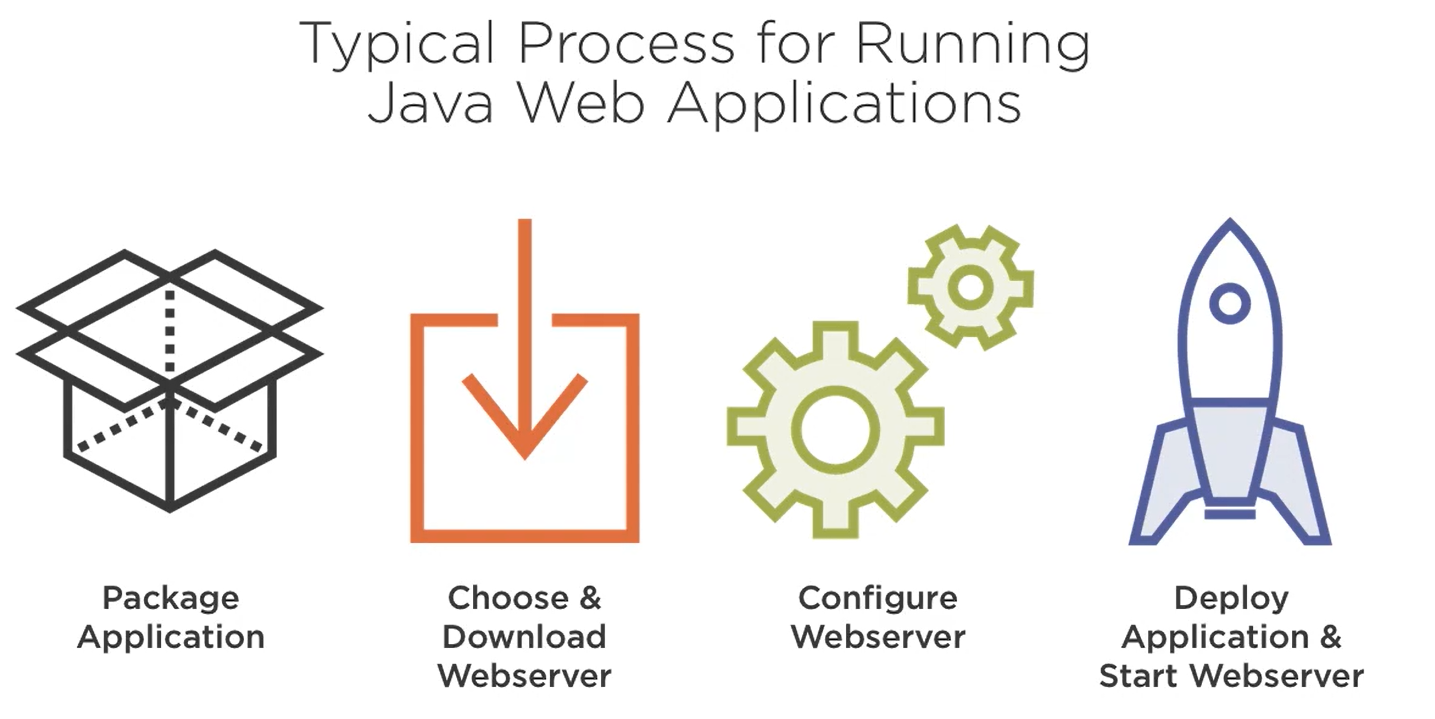
\includegraphics[width=\textwidth]{./images/chapter1/before_spring_boot.png} 

Spring came into being in 2003 as a response to the complexity of the early J2EE specifications. While some consider Java EE and its modern-day successor Jakarta EE to be in competition with Spring, they are in fact complementary. The Spring programming model does not embrace the Jakarta EE platform specification; rather, it integrates with carefully selected individual specifications from the traditional EE umbrella. Spring started as a lightweight alternative to Java Enterprise Edition. Rather than develop components as heavyweight Enterprise
JavaBeans (EJBs), Spring offered a simpler approach to enterprise Java development, utilizing dependency injection and aspect-oriented programming to achieve the capabilities of EJB with plain old Java objects (POJOs).
But while Spring was lightweight in terms of component code, it was heavyweight in terms of configuration. Initially, Spring was configured with XML (and lots of it).
It provides everything you need to create Java enterprise applications. Spring offers the flexibility to create many kinds of architectures depending on an application’s needs. As of Spring Framework 6.0, Spring requires Java 17+.

De lente ontstond in 2003 als reactie op de complexiteit van de vroege J2EE-specificaties. Hoewel sommigen Java EE en zijn moderne opvolger Jakarta EE als concurrenten van Spring beschouwen, zijn ze in feite complementair. Het Spring-programmeringsmodel omarmt niet de Jakarta EE platformspecificatie; in plaats daarvan integreert het met nauwkeurig geselecteerde individuele specificaties uit het traditionele EE-landschap. Spring begon als een lichtgewicht alternatief voor Java Enterprise Edition. In plaats van componenten te ontwikkelen als zware Enterprise JavaBeans (EJB's), bood Spring een eenvoudigere benadering voor enterprise Java-ontwikkeling, waarbij gebruik werd gemaakt van afhankelijkheidsinjectie en aspectgeoriënteerde programmering om de mogelijkheden van EJB te bereiken met gewone Java-objecten (POJO's).
Maar hoewel Spring lichtgewicht was qua componentcode, was het zwaar qua configuratie. In het begin werd Spring geconfigureerd met XML (en veel ervan).
Het biedt alles wat je nodig hebt om Java enterprise-applicaties te maken. Spring biedt de flexibiliteit om verschillende soorten architecturen te creëren, afhankelijk van de behoeften van een applicatie. Vanaf Spring Framework 6.0 vereist Spring Java 17+.

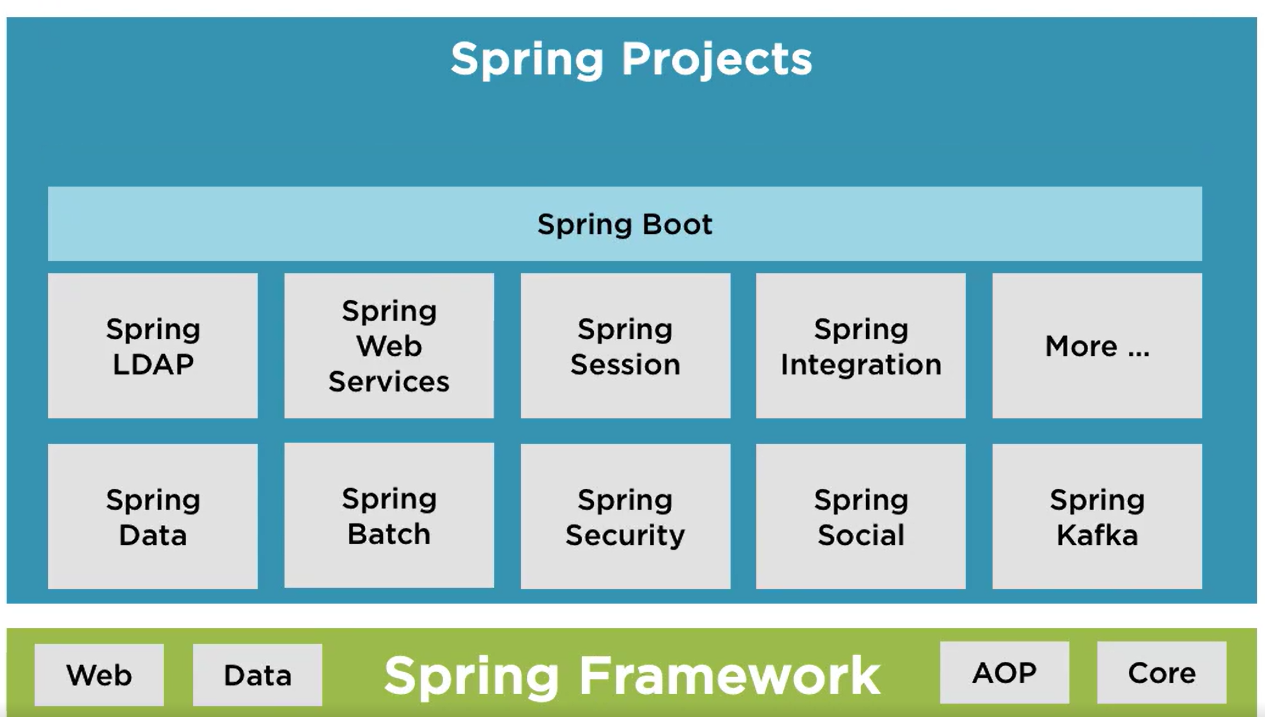
\includegraphics[width=\textwidth]{./images/chapter1/spring_framework.png} 

Spring Boot is a project that is built on the top of the Spring Framework. It provides an easier and faster way to set up, configure, and run java applications.

    
\section{What is Spring Boot?}
 
Spring Boot is an open-source Java framework to create production-ready,  standalone Spring applications. It's a robust, widely used framework. The creation of this framework was facilitated by the desire to simplify the development of applications on the popular Java EE technology stack from Oracle, which was very complex and difficult to use at the time. With very little configuration, you can create easily your first Spring Boot application.

Let's look at some advantages of Spring Boot for developers 
\begin{itemize}
\item speed up the process of creating and deploying application
\item create standalone applications with less or almost no configuration overhead
\item easy to learn framework
\item increase productivity of developers
\end{itemize}

\section{Bootstrapping a simple application}

\subsection{Using Spring Initializr}
Spring Initializr is a web application that can generate a Spring Boot project.
The url for this web application is \url{https://start.spring.io/}. You can select the necessary configuration, including the build tool, language, version of the Spring Boot framework, and any dependencies for your project. IntelliJ IDEA Ultimate provides the Spring Initializr project wizard that integrates with the Spring Initializr API to generate and import your project directly from the IDE.

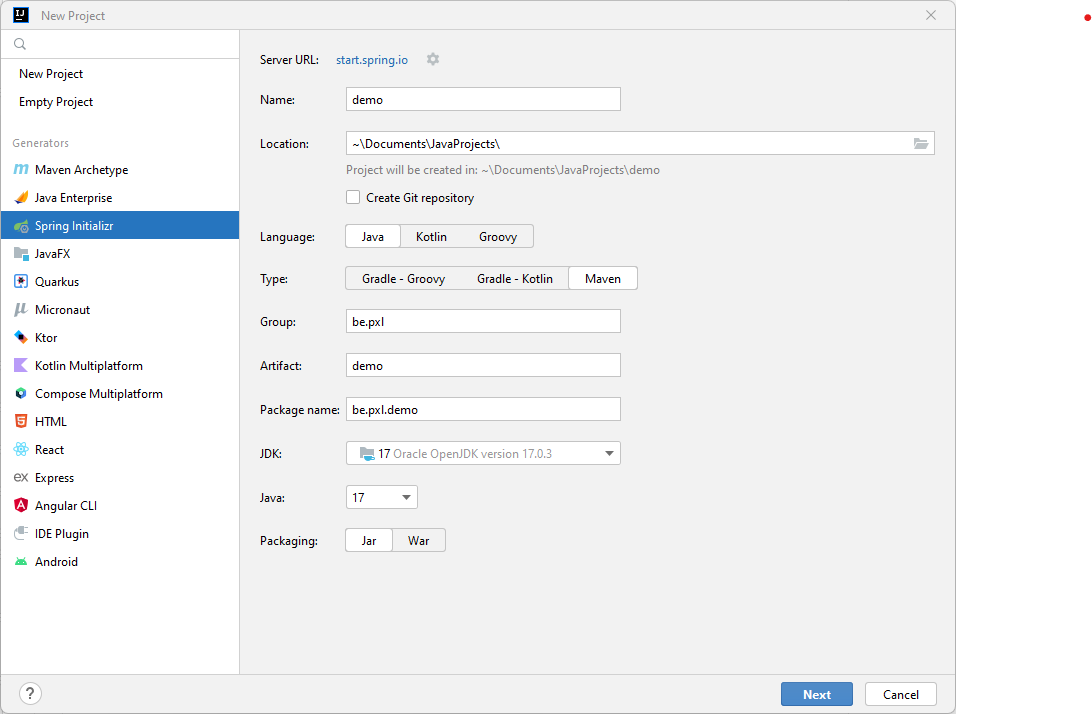
\includegraphics[width=\textwidth]{./images/chapter1/spring_initializer_intellij.png}

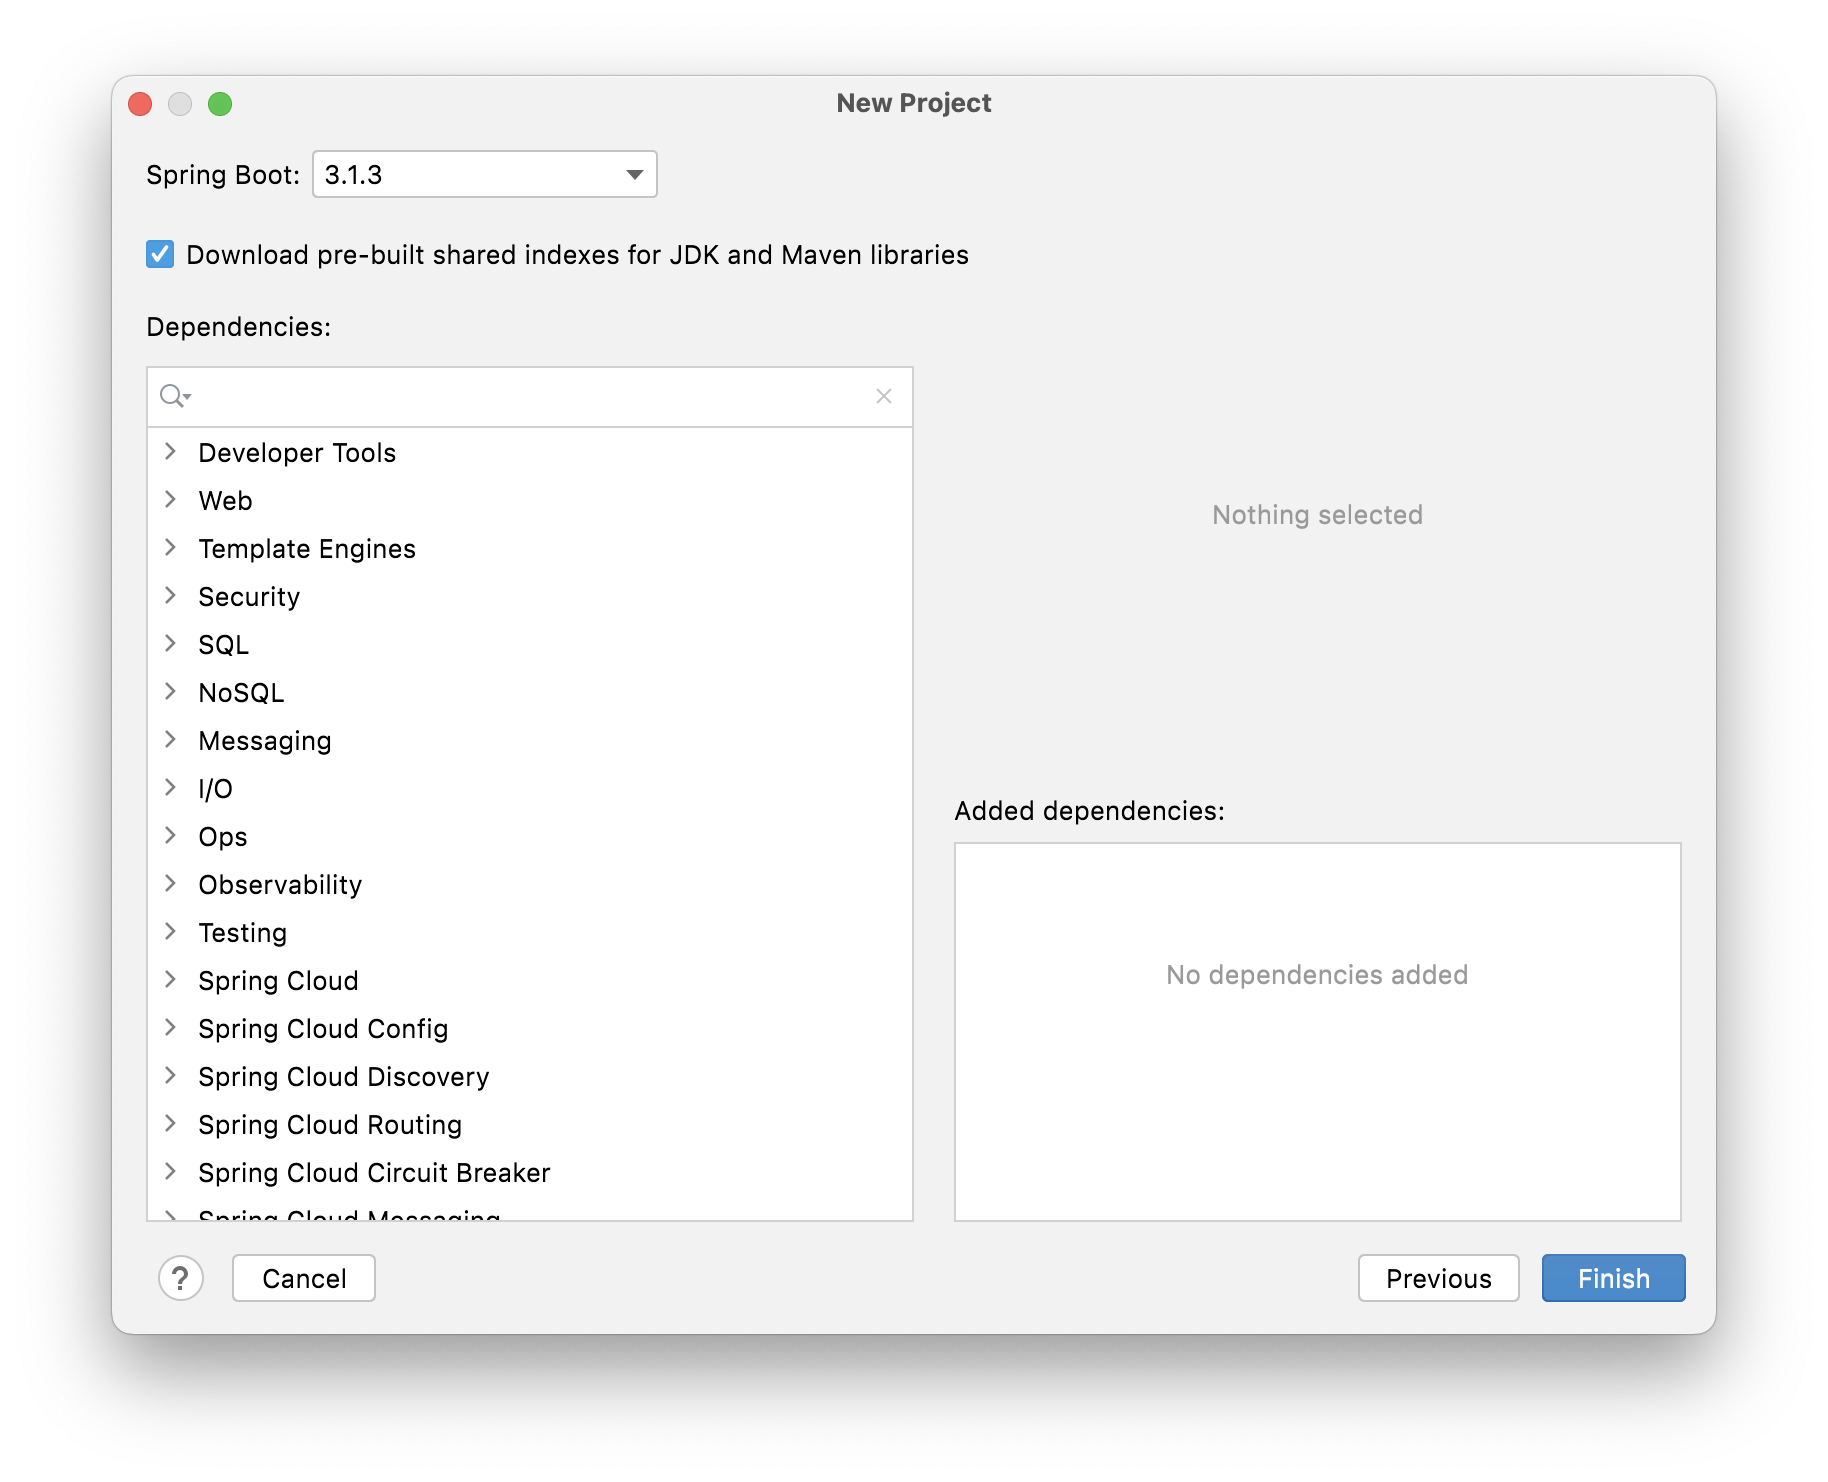
\includegraphics[width=\textwidth]{./images/chapter1/new_project.png}

We select Spring Web dependency. Spring Web uses Spring MVC. It is used for building RESTful Web Services. Spring MVC provides the annotation @RestController for classes that implement the REST endpoints.
To run a RESTful Web Service you need a web container. Spring Boot will automatically add an embedded Tomcat web container to your project. If you prefer another web container, you can update Spring Boot's configuration.
Finally Jackson is a popular third-party library for converting Java-objects to JSON and vice versa.

\begin{oefening}
Create the demo project. You can use the wizard in IntelliJ IDEA Ultimate or \url{https://start.spring.io/}.
\end{oefening}

\section{Running the demo project}

The starting point of a Spring Boot application is the class with the main-method and annotated with @SpringBootApplication.  This class can be found in the folder /src/main/java.  Spring Boot offers a lot of annotations to reduce the workload of developers.   

\begin{lstlisting}[frame=single]
package be.pxl.demo;

import org.springframework.boot.SpringApplication;
import org.springframework.boot.autoconfigure.SpringBootApplication;

@SpringBootApplication
public class DemoApplication {

    public static void main(String[] args) {
        SpringApplication.run(DemoApplication.class, args);
    }

}
\end{lstlisting}

By running the main-class you start your Spring Boot application. 

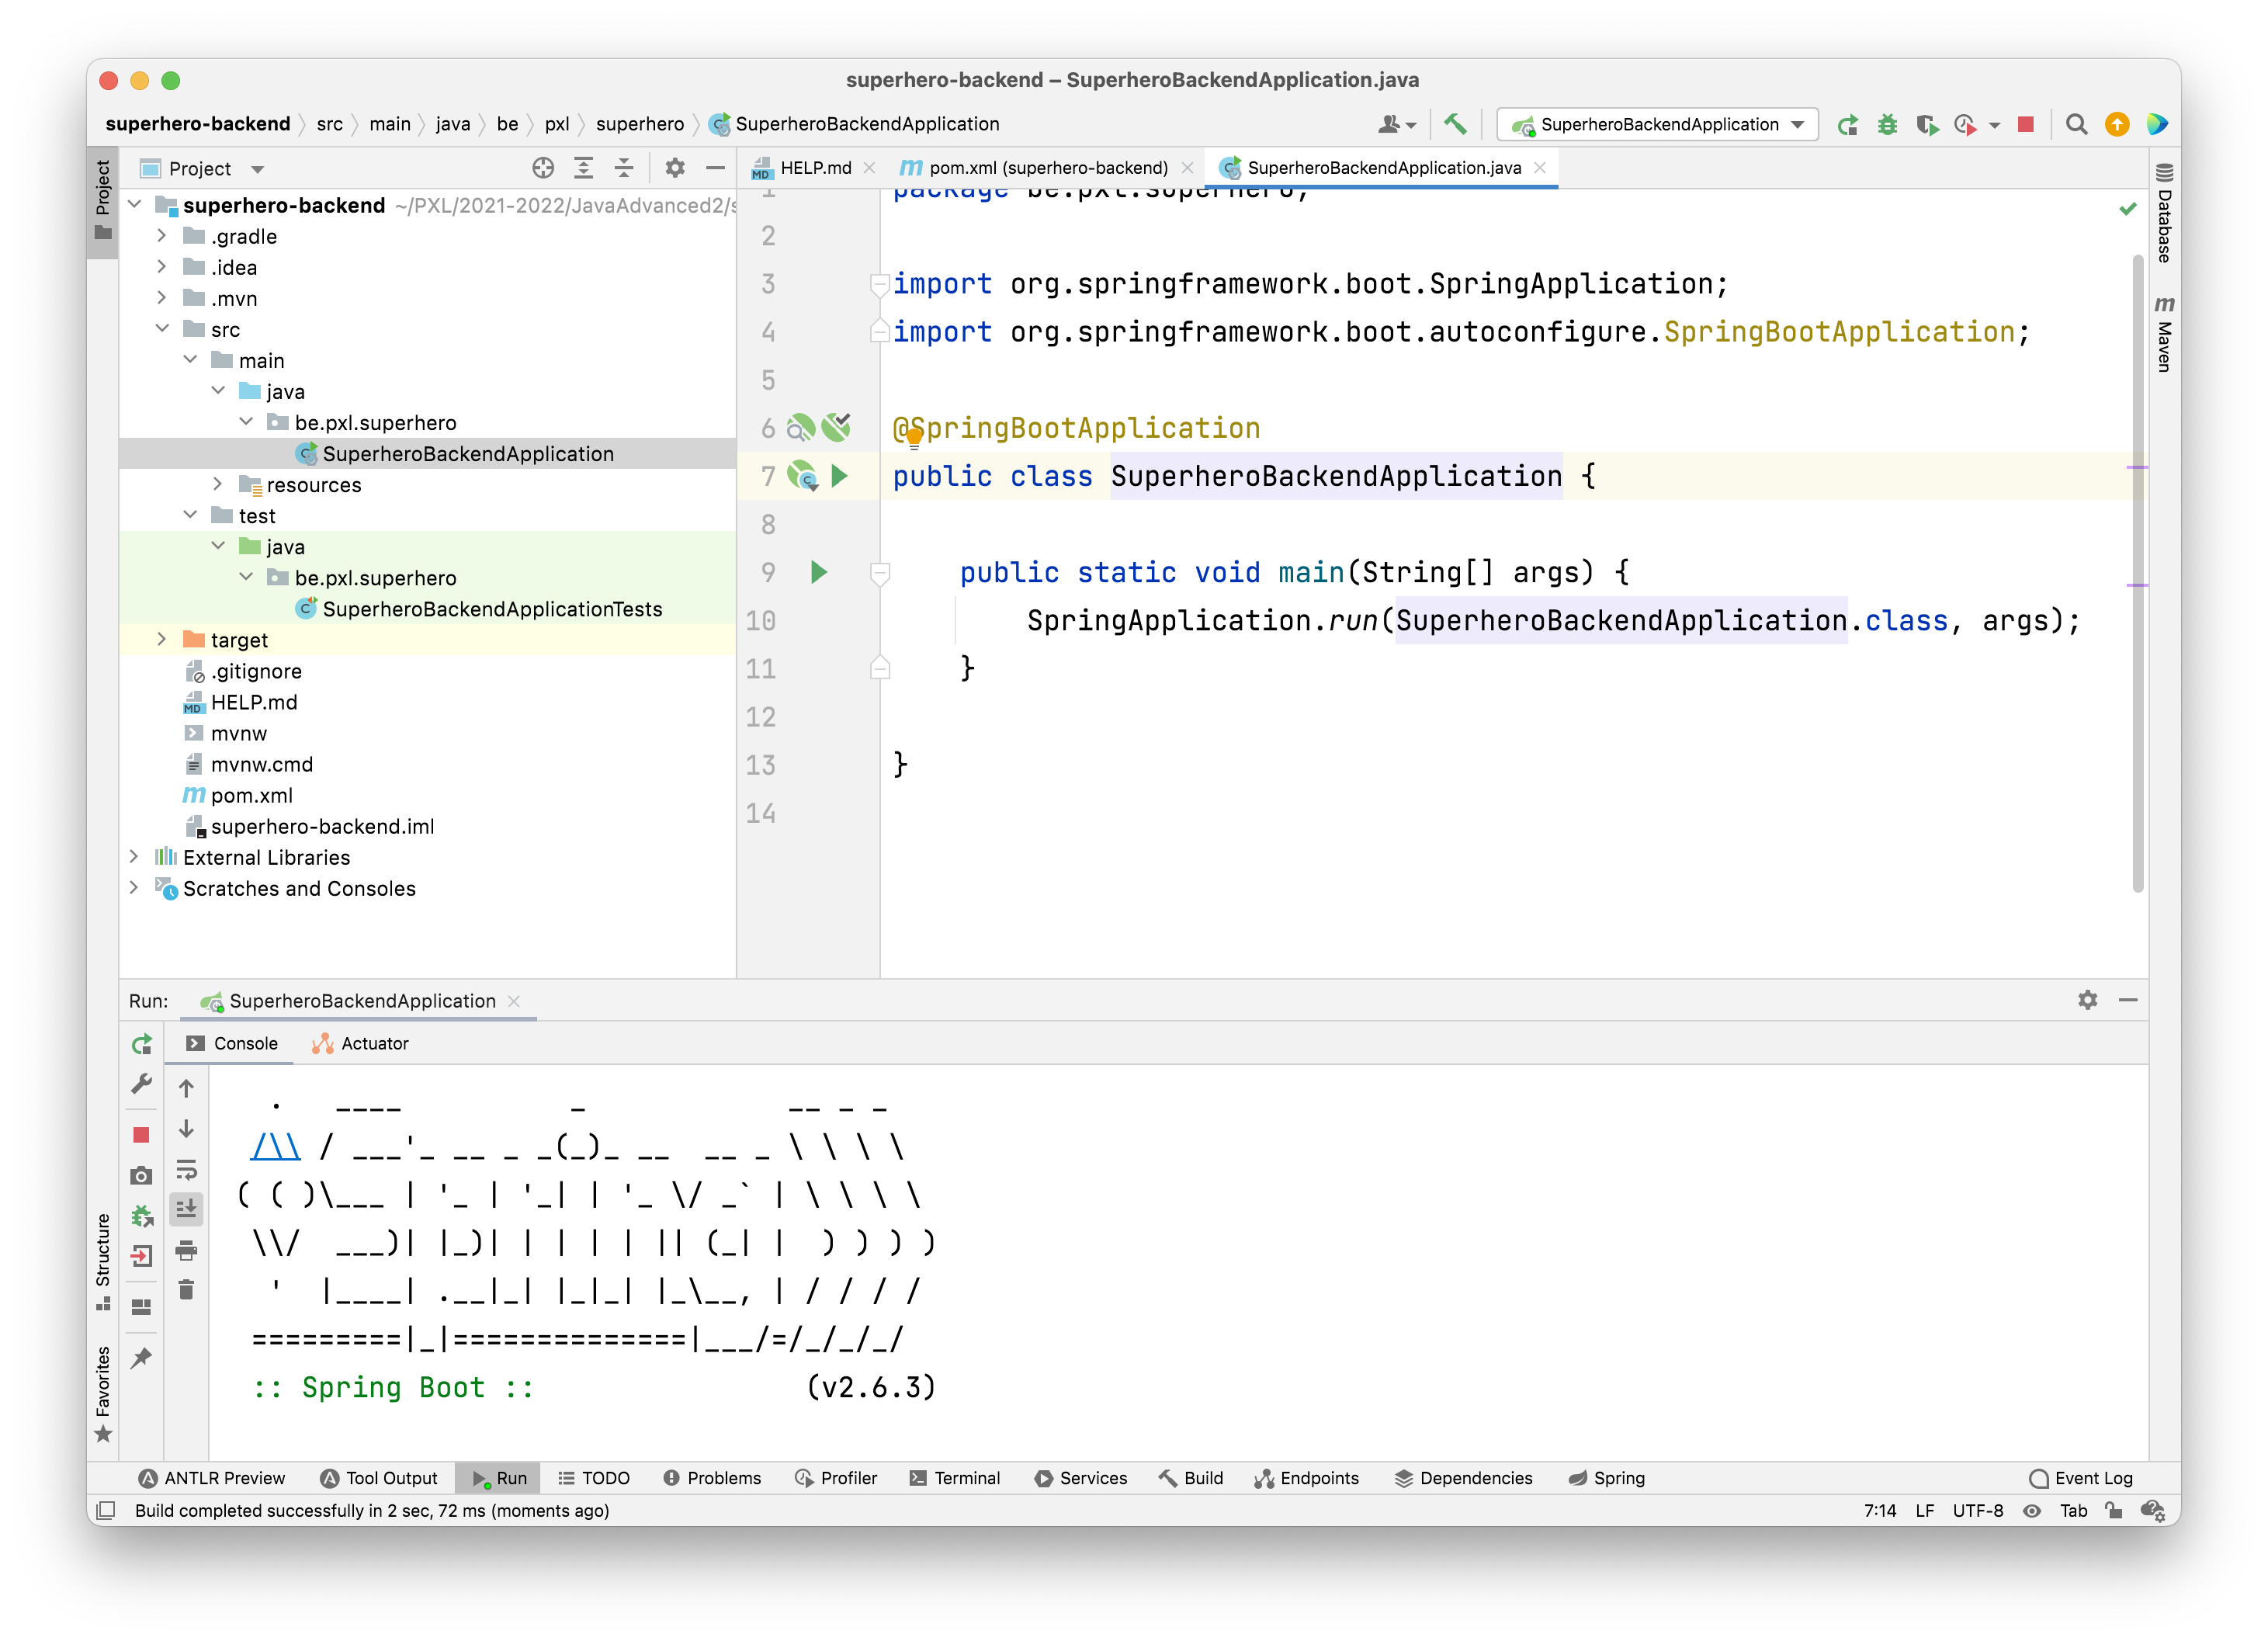
\includegraphics[width=\textwidth]{./images/chapter2/first-run.png}

Currently our Spring Boot application only shows a whitelabel error page. This error page is available when you perform a GET for URL \url{http://localhost:8080}.

\frame{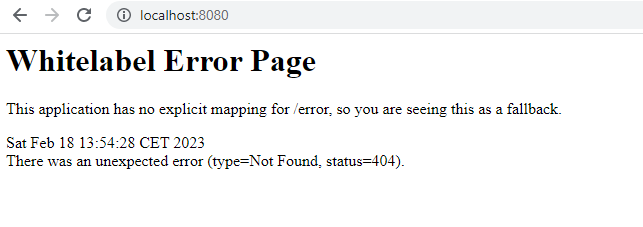
\includegraphics[width=\textwidth]{./images/chapter2/whitelabel_error_page.png}} 

Port 8080 is the default port. If this port is not available you will see an error message in Spring Boot's logging.

\begin{lstlisting}[frame=single]
***************************
APPLICATION FAILED TO START
***************************

Description:

Web server failed to start. Port 8080 was already in use.
\end{lstlisting}

The port number can be changed in the file application.properties. You have to add the property server.port here with the desired port number.

\begin{lstlisting}[frame=single]
server.port=8081
\end{lstlisting}

\subsection{Component}


\begin{lstlisting}
@Component
public class DependencyInjectionWithSpring implements CommandLineRunner {
   
   @Override    
   public void run(String... args) throws Exception {
	   System.out.println("Welcome to Java Advanced");
   }
}
\end{lstlisting}

De Spring Boot de CommandLineRunner interface voorziet de mogelijkheid om een stukje code uit te voeren zodra de Spring Boot applicatie ge\"initialiseerd is. 

Zodra je de CommandLineRunner interface implementeert in een klasse kan je de run-methode overschrijven. In de run-methode plaats je de code die uitgevoerd moet worden
als de applicatie opstart.  Zodra de Spring Boot applicatie opstart worden een aantal initialisatie-fasen doorlopen.  Eerst wordt de \textbf{application context} aangemaakt en alle Spring beans worden geladen. Als de applicatie volledige is ge\"initialiseerd wordt de run-methode van de CommandLineRunner automatisch door het Spring boot framework aangeroepen.



\subsubsection{Spring beans}

Spring Beans zijn componenten die volledig worden beheerd door het Spring Boot framework. Je hoeft zelf geen instanties van deze klassen te maken, Spring Boot genereert de objecten automatisch.  Daarnaast beheert Spring Boot ook de objecten. Wanneer een klasse gebruik wil maken van de functionaliteiten van een dergelijke Spring Bean, zal Spring Boot ervoor zorgen dat de instantie van de Spring Bean beschikbaar is voor de betreffende klasse.

\subsubsection{Application context}

De Application context is een belangrijk onderdeel van elke Spring Boot applicatie.
Hierin wordt namelijk bijgehouden welke infals een slimme doos waarin alle informatie en instellingen voor je Spring Boot-toepassing worden bewaard. Deze doos zorgt ervoor dat alle onderdelen van je applicatie met elkaar kunnen praten en weten waar ze moeten zoeken voor dingen zoals configuratie, gegevensbronnen en andere beans (componenten). Het maakt je Spring Boot-applicatie georganiseerd en helpt deze soepel te werken door alles op één plek te houden. Je kunt de application context beschouwen als het brein van je Spring Boot-applicatie dat alles coördineert en beschikbaar maakt voor de verschillende onderdelen van je programma.


Iets meer info tonen:

spring.application.name=My Demo

package be.pxl.demo.beans;

import org.springframework.boot.CommandLineRunner;
import org.springframework.context.ApplicationContext;
import org.springframework.stereotype.Component;

import java.time.LocalDateTime;
import java.time.ZoneId;
import java.time.ZoneOffset;

@Component
public class DependencyInjectionWithSpring implements CommandLineRunner {
	private final ApplicationContext applicationContext;

	public DependencyInjectionWithSpring(ApplicationContext applicationContext) {
		this.applicationContext = applicationContext;
	}

	@Override
   public void run(String... args) throws Exception {
	   System.out.println("Welcome to Java Advanced");
		System.out.println(applicationContext.getApplicationName());
		System.out.println(applicationContext.getDisplayName());
		System.out.println(applicationContext.getId());
		LocalDateTime dateTime = convertStartupDateToLocalDateTime(applicationContext.getStartupDate());
		System.out.println(dateTime);
		System.out.println(LocalDateTime.now());
   }


   private LocalDateTime convertStartupDateToLocalDateTime(long startupDate) {
	   // Get the system's default timezone
	   ZoneId systemZoneId = ZoneId.systemDefault();
	   // Get the ZoneOffset for the system's default timezone
	   ZoneOffset systemZoneOffset = systemZoneId.getRules().getOffset(LocalDateTime.now());
		return LocalDateTime.ofEpochSecond(applicationContext.getStartupDate() / 1000, 0, systemZoneOffset);

   }
}



Spring Boot Application Context:
When your Spring Boot application starts, it goes through various phases of initialization. After the application context is prepared and all beans are loaded, any classes implementing CommandLineRunner are executed.

\subsection{The Maven pom file}

POM stands for \'Project Object Model\'. It is an XML representation of a Maven project held in a file named pom.xml. This file can be found in your project directory. The POM contains all necessary information about a project, as well as configurations of plugins to be used during the build process. We will cover Maven in chapter 3.

\begin{lstlisting}[frame=single]
<?xml version="1.0" encoding="UTF-8"?>
<project xmlns="http://maven.apache.org/POM/4.0.0" xmlns:xsi="http://www.w3.org/2001/XMLSchema-instance"
         xsi:schemaLocation="http://maven.apache.org/POM/4.0.0 https://maven.apache.org/xsd/maven-4.0.0.xsd">
    <modelVersion>4.0.0</modelVersion>
    <parent>
        <groupId>org.springframework.boot</groupId>
        <artifactId>spring-boot-starter-parent</artifactId>
        <version>3.0.2</version>
        <relativePath/> <!-- lookup parent from repository -->
    </parent>
    <groupId>be.pxl</groupId>
    <artifactId>demo</artifactId>
    <version>0.0.1-SNAPSHOT</version>
    <name>demo</name>
    <description>demo</description>
    <properties>
        <java.version>17</java.version>
    </properties>
    <dependencies>
        <dependency>
            <groupId>org.springframework.boot</groupId>
            <artifactId>spring-boot-starter-web</artifactId>
        </dependency>

        <dependency>
            <groupId>org.springframework.boot</groupId>
            <artifactId>spring-boot-starter-test</artifactId>
            <scope>test</scope>
        </dependency>
    </dependencies>

    <build>
        <plugins>
            <plugin>
                <groupId>org.springframework.boot</groupId>
                <artifactId>spring-boot-maven-plugin</artifactId>
            </plugin>
        </plugins>
    </build>
</project>
\end{lstlisting}

spring-boot-starter-parent is a starter project that provides the default configuration for spring-based applications. Here you choose the version of Spring Boot.

For large projects, managing the dependencies is not always easy. Spring Boot solves this problem by grouping certain dependencies together. These groups of dependencies are called starters. All Spring Boot starters are named following the same naming pattern. The all start with spring-boot-starter-*, where * indicates the purpose and functionality provided by the starter.

spring-boot-starter-web adds all the libraries we need to develop web components. An embedded server will be provided in the Spring Boot project. Therefore the environment where the Spring Boot project is executed does not need to have a pre-installed server. The default embedded server for Spring Boot is Tomcat. The Spring MVC framework which provides all classes for developing RESTful web services is also part of spring-boot-starter-web.

spring-boot-starter-test (with scope test) is the starter for testing Spring Boot applications with libraries including JUnit Jupiter, Hamcrest and Mockito.

Inversion of Control (IoC) is \'e\'en van de basisprincipes van het Spring framework.
Bij Inversion of Control is het aanmaken en beheren van objecten niet langer de verantwoordelijkheid van de objecten zelf, maar is er een aparte 

So, Inversion of Control is about shifting the responsibility of managing object interactions from your code to a higher-level component (the framework or container). This makes your code more modular and flexible, as you rely on the framework to provide and coordinate the necessary components, 

To explain this in layman's terms, suppose you drive a car to your work place. This means you control the car. The IoC principle suggests to invert the control, meaning that instead of driving the car yourself, you hire a cab, where another person will drive the car.

What is a Bean in Spring Boot? A Bean is an object that is managed by the Spring framework. It is created, managed, and managed by the Spring container. Beans can be used to encapsulate and provide services, utilities, and functionalities to other components in an application.

In Spring, the objects that form the backbone of your application and that are managed by the Spring IoC container are called beans. A bean is an object that is instantiated, assembled, and otherwise managed by a Spring IoC container. Otherwise, a bean is simply one of many objects in your application.

TODO add image





IOC en dependency injection 


@Component
public class DependencyInjectionWithSpring implements CommandLineRunner {
   
   @Autowired
   private WeatherService weatherService;
   
   @Override    
   public void run(String... args) throws Exception {
	   weatherService.printWeather();
   }
}

WeatherService.java

import org.springframework.stereotype.Component;

@Component
public class WeatherService {
   public void printWeather() {
      System.out.println("The weather is sunny with a 20% chance of rain");
   }
}


Exercise

Create the class 





\subsection{@SpringBootApplication}

Java annotations are a mechanism for adding metadata information to our source code. An annotation processor processes these annotations at compile time or runtime to provide functionality such as code generation, error checking, etc.

@SpringBootApplication annotation is used to enable following three features:
\begin{itemize}
\item @EnableAutoConfiguration: enable Spring Boot’s auto-configuration mechanism
\item @ComponentScan: enable @Component scan on the package where the application is located
\item @Configuration: allow to register extra beans in the context or import additional configuration classes
\end{itemize}


\subsection{Auto-configuration}

Spring Boot auto-configuration attempts to automatically configure your Spring application based on the dependencies that you have added.
To gain some insight in this auto-configuration let's add a line in the application.properties file. This file can be found in the directory /src/main/resources. 

\begin{lstlisting}
logging.level.org.springframework=debug
\end{lstlisting}

logging.level.org.springframework is a application properties. A list of all available application properties can be found at \url{https://docs.spring.io/spring-boot/docs/current/reference/html/application-properties.html}.

\begin{oefening}
Add the line above to the application.properties file and restart the Spring Boot application.
\end{oefening}

In the console you will find all the auto-configuration Spring Boot is doing.

\chapter{REST}

\fcolorbox{black}[HTML]{E9F0E9}{\parbox{\textwidth}{%
\noindent \textbf{Learning goals}\\
De junior-collega
\begin{enumerate}[nolistsep]
\item kan beschrijven wat een RESTful web applicatie is
\item kan een POST, GET, PUT en DELETE-verzoek afhandelen in Spring Boot
\item kan beschrijven wat spring-boot-starter-web is
\item 
\end{enumerate}}}

\section{HTTP-verzoekmethoden}

Spring Boot is een goede keuze als je een REST API (of voluit een RESTful web API) wilt ontwikkelen in Java.

REST (Representational State Transfer) is een gestandaardiseerde manier om communicatie tussen verschillende softwaretoepassingen over het internet mogelijk te maken. 
In een RESTful web applicatie wordt de functionaliteit van de applicatie beschikbaar gesteld als resources, die kunnen worden geïdentificeerd door URI's (Uniform Resource Identifiers).  Gebruikers en andere applicaties kunnen met deze resources communiceren via standaard HTTP-verzoekmethoden (HTTP-request, HTTP-method of HTTP-verb). In essentie is HTTP het transportprotocol dat wordt gebruikt om gegevens over te dragen,  terwijl REST de verzameling van ontwerpprincipes is die bepalen hoe die gegevens moeten worden georganiseerd en benaderd.

\begin{itemize}
\item \textbf{GET}: Het GET-verzoek wordt gebruikt om gegevens op te halen van een specifieke resource. 

Voorbeeld URI: GET /api/products/123

Dit verzoek haalt informatie op over het product met ID 123.

\item \textbf{POST}: Het POST-verzoek wordt gebruikt om nieuwe gegevens naar een resource te verzenden. Het wordt vaak gebruikt voor het maken van nieuwe resources of het toevoegen van gegevens aan een bestaande resource.

Voorbeeld URI: POST /api/products

Dit verzoek voegt een nieuw product toe aan de lijst van producten.

\item \textbf{PUT}: Het PUT-verzoek wordt gebruikt om gegevens bij te werken voor een specifieke resource of om een nieuwe resource te maken als deze niet bestaat. Het is idempotent, wat betekent dat meerdere PUT-verzoeken hetzelfde resultaat opleveren.

Voorbeeld URI: PUT /api/products/123

Dit verzoek bijwerken de informatie van het product met ID 123.

\item \textbf{DELETE}: Het DELETE-verzoek wordt gebruikt om een resource te verwijderen of te deactiveren.

Voorbeeld URI: DELETE /api/products/123

Dit verzoek verwijdert het product met ID 123 uit de lijst van producten.
\end{itemize}

\section{Spring Boot Starter Web}

Spring Boot Starter Web is de verzameling van alle bibliotheken (third party libraries) die we nodig hebben om RESTful web applicaties te bouwen.  De verzameling bestaat ondermeer uit Spring MVC,  REST,  jackson en Tomcat. 
Apache Tomcat is een populaire open source web server voor Java toepassingen.  Als je de dependency spring-boot-start-web toevoegt, start de Tomcat web server op zodra je de Spring boot applicatie opstart.  We spreken van de "embedded web server" in Spring boot.  Je kan er ook voor kiezen om  \'e\'en van de alternatieve web servers te gebruiken zoals jetty of undertow. 
Jackson is een populaire library om Java-objecten naar JSON te converteren en vice versa.

\begin{lstlisting}
<dependency>
		<groupId>org.springframework.boot</groupId>
		<artifactId>spring-boot-starter-web</artifactId>
</dependency>
\end{lstlisting}
		
Je voegt de dependency toe in het bestand pom.xml.
		
Start nu de Spring Boot applicatie opnieuw op.

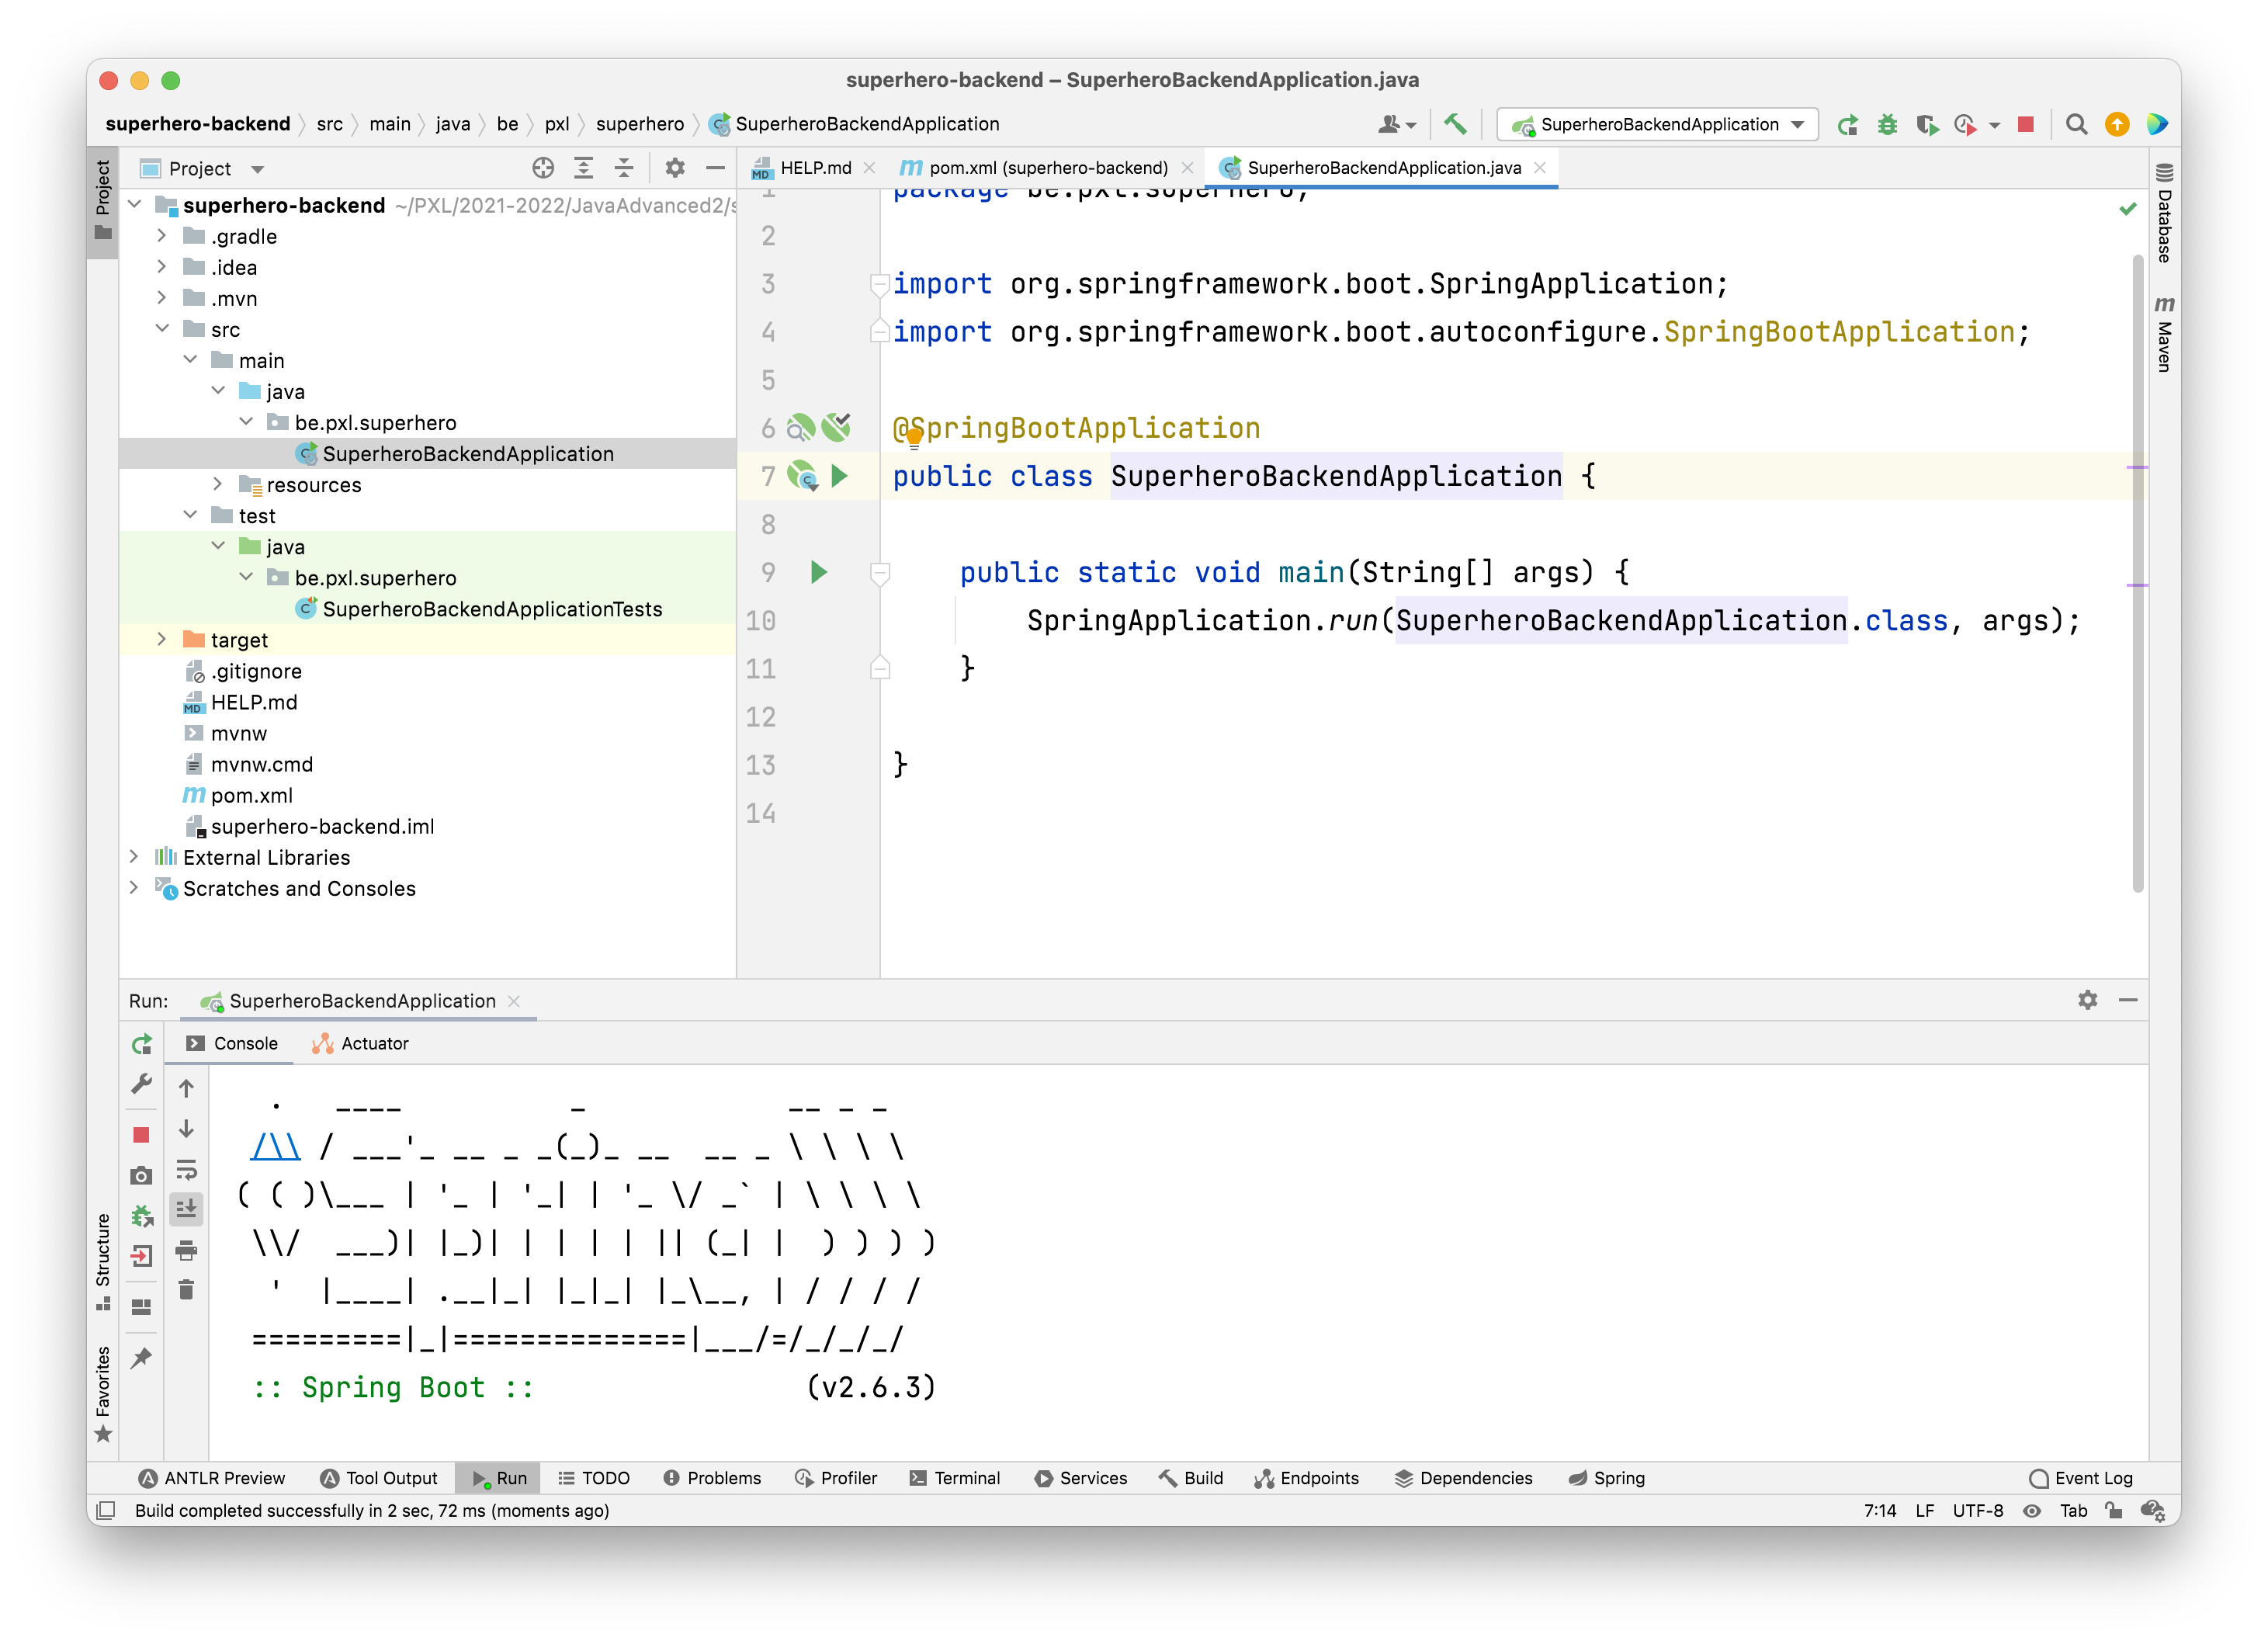
\includegraphics[width=\textwidth]{./images/chapter2/first-run.png}

Momenteel kan de Spring Boot applicatie enkel een whitelabel error pagina tonen.  De error pagina krijg je te zien als je een GET-request uitvoert voor URL \url{http://localhost:8080}.

\frame{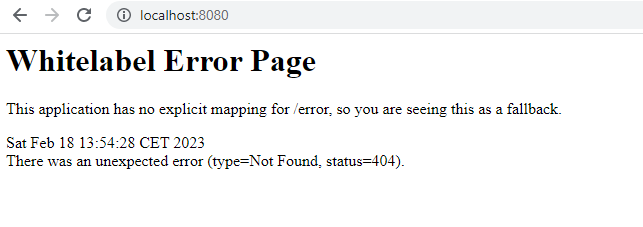
\includegraphics[width=\textwidth]{./images/chapter2/whitelabel_error_page.png}} 

Poort 8080 is de default poort van de Tomcat webserver.  Als deze poort al gebruikt wordt door een ander programma, krijg je de volgende foutmelding te zien.

\begin{lstlisting}[frame=single]
***************************
APPLICATION FAILED TO START
***************************

Description:

Web server failed to start. Port 8080 was already in use.
\end{lstlisting}

De poortnummer kan aangepast worden in het bestand application.properties.  Je gebruikt de eigenschap \textbf{server.port} om de gewenste poortnummer te kiezen.

\begin{lstlisting}[frame=single]
server.port=8081
\end{lstlisting}

\section{De RestController}

Spring boot heeft een annotatie voorzien voor de Spring bean die verantwoordelijk is voor het afhandelen van HTTP requests nl. @RestController. Spring boot heeft ook een annotatie @Controller, maar de @RestController zorgt ervoor dat het respons op het HTTP-request automatisch wordt omgezet (geserialiseerd) naar JSON of XML en wordt teruggestuurd naar de client.


\begin{lstlisting}[frame=single]
package be.pxl.demo.api;

import jakarta.annotation.PostConstruct;
import org.springframework.web.bind.annotation.GetMapping;
import org.springframework.web.bind.annotation.RestController;

import java.util.ArrayList;
import java.util.List;
import java.util.Random;

@RestController
@RequestMapping("/greetings")
public class GreetingController {

    private final List<String> messages = new ArrayList<>();
    private static final Random RANDOM = new Random();

    @PostConstruct
    public void init() {
        messages.add("Peek-a-boo!");
        messages.add("Howdy-doody!");
        messages.add("My name's Ralph, and I'm a bad guy.");
        messages.add("I come in peace!");
        messages.add("Put that cookie down!");

    }

    @GetMapping("/hello")
    public String doGreeting() {
        return messages.get(RANDOM.nextInt(messages.size()));
    }
}
\end{lstlisting}

De @RestController markeert de klasse GreetingController als een REST-controller.
De annotatie @RequestMapping("/greetings") specificeert het basispad voor alle requests die door deze controller worden afgehandeld.
@GetMapping("/hello") geeft aan dat de goGreeting-methode wordt uitgevoerd wanneer een HTTP GET-verzoek wordt gemaakt naar het pad "/greetings/hello". Het resultaat van deze methode wordt automatisch omgezet in tekst en teruggestuurd als de respons.

\begin{figure}[H]
  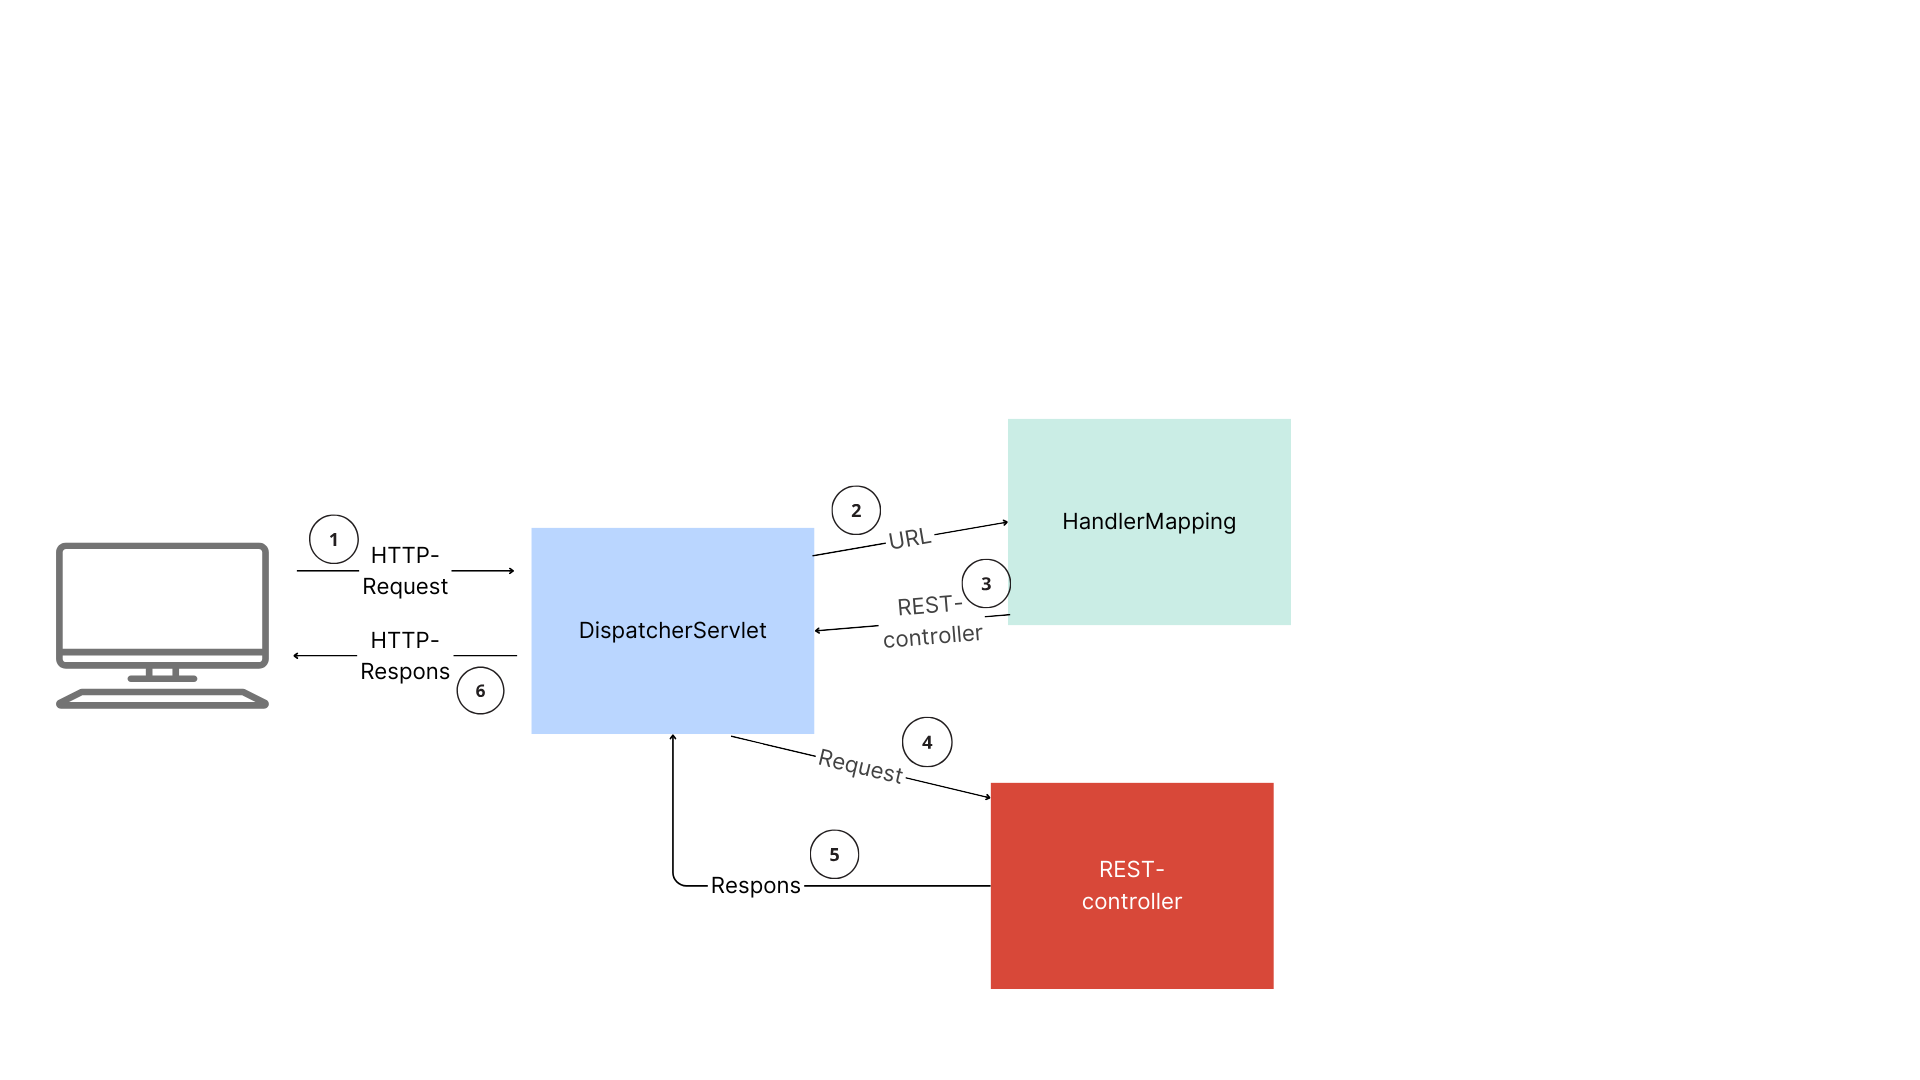
\includegraphics[width=\linewidth]{images/chapter-rest/dispatcherservlet.png}
  \caption{Een REST-verzoek afhandelen}
  \label{fig:test_passed}
\end{figure}

De component van Spring Boot die verantwoordelijk is dat een HTTP-request door de juiste REST-controller wordt afgehandeld is de DispatcherServlet.  De DispatcherServlet is onderdeel van Spring MVC.  De DispatcherServlet bepaalt welke controller een HTTP-request moet afhandelen,  hij geeft het request door aan de juiste controller en  verwerkt het respons van de controller om een HTTP-respons terug te sturen naar de client.

Om te achterhalen welke REST-controller verantwoordelijk is om een HTTP-request af te handelen raadpleegt de DispatcherServlet de HandlerMapping. De HandlerMapping is als het ware een kaart die URL's koppelt aan specifieke controllerklassen en methoden.
Op basis van de URL in het binnenkomende request bepaalt de DispatcherServlet welke controllerklasse en methode verantwoordelijk zijn voor het afhandelen van het request.


\begin{oefening}
Maak het package \textit{be.pxl.demo.api}.  Voeg de klasse \textbf{GreetingController} toe het package.  Start de Spring Boot applicatie en open de URL \url{http://localhost:8080/greetings/hello} in een browser. Voeg in de REST-controller een methode toe met de URI GET /greetings/daytime die de huidige dag en het tijdstip teruggeeft in het formaat 'Maandag 18 september 2023'.
\end{oefening}

\section{MusicPlaylist}

We gaan een nieuwe Spring Boot toepassing aanmaken waarmee we een muziek playlist beheren. 

\begin{oefening}
Maak een nieuwe Spring boot toepassing MusicPlaylist. We gebruiken Spring MVC om een RESTful web applicatie te maken.  
\end{oefening}

\subsection{Een liedje toevoegen aan een playlist}

\begin{apiRoute}{post}{/playlist/songs}{Add a new song to the playlist.}
\begin{routeRequest}{application/json}
\begin{routeRequestBody}
{
  "title": "Hello",
  "artist": "Adele",
  "duration_seconds": 293,
  "genre": "POP"
}
\end{routeRequestBody}
\end{routeRequest}
\begin{routeResponse}{application/json}
\begin{routeResponseItem}{200}{ok}
\end{routeResponseItem}
\end{routeResponse}
\end{apiRoute}


Om te beginnen hebben we de klasse Song nodig. 

\begin{lstlisting}[language=java,  frame=single]
public class Song {
    private String title;
    private String artist;
    @JsonProperty("duration_seconds")
    private int durationSeconds;
    private Genre genre;

    // Default constructor
    public Song() {
    }

    // Parameterized constructor
    public Song(String title, String artist, int durationSeconds, Genre genre) {
        this.title = title;
        this.artist = artist;
        this.durationSeconds = durationSeconds;
        this.genre = genre;
    }

    // Getter and setter methods
    public String getTitle() {
        return title;
    }

    public void setTitle(String title) {
        this.title = title;
    }

    public String getArtist() {
        return artist;
    }

    public void setArtist(String artist) {
        this.artist = artist;
    }

    public int getDurationSeconds() {
        return durationSeconds;
    }

    public void setDurationSeconds(int durationSeconds) {
        this.durationSeconds = durationSeconds;
    }

    public Genre getGenre() {
        return genre;
    }

    public void setGenre(Genre genre) {
        this.genre = genre;
    }

    @Override
    public String toString() {
        return "Song{" +
                "title='" + title + '\'' +
                ", artist='" + artist + '\'' +
                ", durationSeconds=" + durationSeconds +
                ", genre='" + genre + '\'' +
                '}';
    }
}
\end{lstlisting}


Nu gaan we de REST-controller implementeren.  We gaan hierin een methode voorzien die een POST op de URI /playlist/songs kan afhandelen.  Initieel gaan we enkel de titel in de loggegevens tonen. 

\begin{lstlisting}[language=java,  frame=single]
@RestController
@RequestMapping("/playlist/songs")
public class MusicPlaylistController {

	private static final Logger LOGGER = LoggerFactory.getLogger(MusicPlaylistController.class);

	@PostMapping
	public void addSong(@RequestBody Song song) {
		if (LOGGER.isInfoEnabled()) {
			LOGGER.info("Adding song [" + song.getTitle() + "]");
		}
	}
}
\end{lstlisting}

De liedjes die aan de playlist worden toegevoegd willen we bijhouden. Later zullen we ze wegschrijven in een databank, maar voorlopig gaan we ze bijhouden in een lijst.
Om dit mogelijk te maken gaan we een nieuwe Spring Bean toevoegen: de MusicPlaylistService.  

\begin{lstlisting}[language=java,  frame=single]
package be.pxl.demo;

import be.pxl.demo.domain.Song;
import org.springframework.stereotype.Service;

import java.util.ArrayList;
import java.util.List;

@Service
public class MusicPlaylistService {
	private final List<Song> myPlaylist = new ArrayList<>();

	public void addSong(Song song) {
		myPlaylist.add(song);
	}
}
\end{lstlisting}

De MusicPlaylistService wordt geannoteerd met @Service .
In onze Spring Boot applicaties gaan we steeds de business-logica implementeren in de service-laag.  De @Service annotatie wordt gebruikt voor de componenten (Spring Beans) in de service-laag.  Wanneer onze Spring Boot applicatie opstart wordt er exact \'e\'en instantie van de MusicPlaylistService aangemaakt in de ApplicationContext en deze instantie wordt tijdens de volledige levensduur van de toepassing gebruikt.  Dit noemen we de scope van de service en de default scope noemen we \textbf{singleton}. 
Dit betekent dat we \'e\'en enkele, gedeelde playlist hebben voor alle gebruikers.

Nu gaan we de MusicPlaylistService beschikbaar maken in de MusicPlaylistController.
We maken gebruik van \textbf{constructor injection}.  Zodra de instantie van de MusicPlaylistController door Spring Boot wordt aangemaakt, zal er eerst gezorgd worden dat de instantie MusicPlaylistService aangemaakt wordt. Deze instantie wordt dan achter de schermen meegegeven aan de constructor van de MusicPlaylistController. Zo kan ons MusicPlaylistController-object het MusicPlaylistService-object gebruiken.
Omdat er maar \'e\'en constructor is, is de annotatie @Autowired eigenlijk overbodig.

\begin{lstlisting}[language=java,  frame=single]
@RestController
@RequestMapping("/playlist/songs")
public class MusicPlaylistController {

	private static final Logger LOGGER = LoggerFactory.getLogger(MusicPlaylistController.class);
	private final MusicPlaylistService musicPlaylistService;

	@Autowired
	public MusicPlaylistController(MusicPlaylistService musicPlaylistService) {
		this.musicPlaylistService = musicPlaylistService;
	}

	@PostMapping
	public void addSong(@RequestBody Song song) {
		if (LOGGER.isInfoEnabled()) {
			LOGGER.info("Adding song [" + song.getTitle() + "]");
		}
		musicPlaylistService.addSong(song);
	}
}
\end{lstlisting}

Test nu het POST-verzoek.  Je kan Postman,  Insomnia of een andere tool gebruiken om een POST-verzoek naar de toepassing te sturen.  De toegevoegde liedjes gaan uiteraard verloren wanneer je de toepassing herstart. 

\begin{figure}[H]
  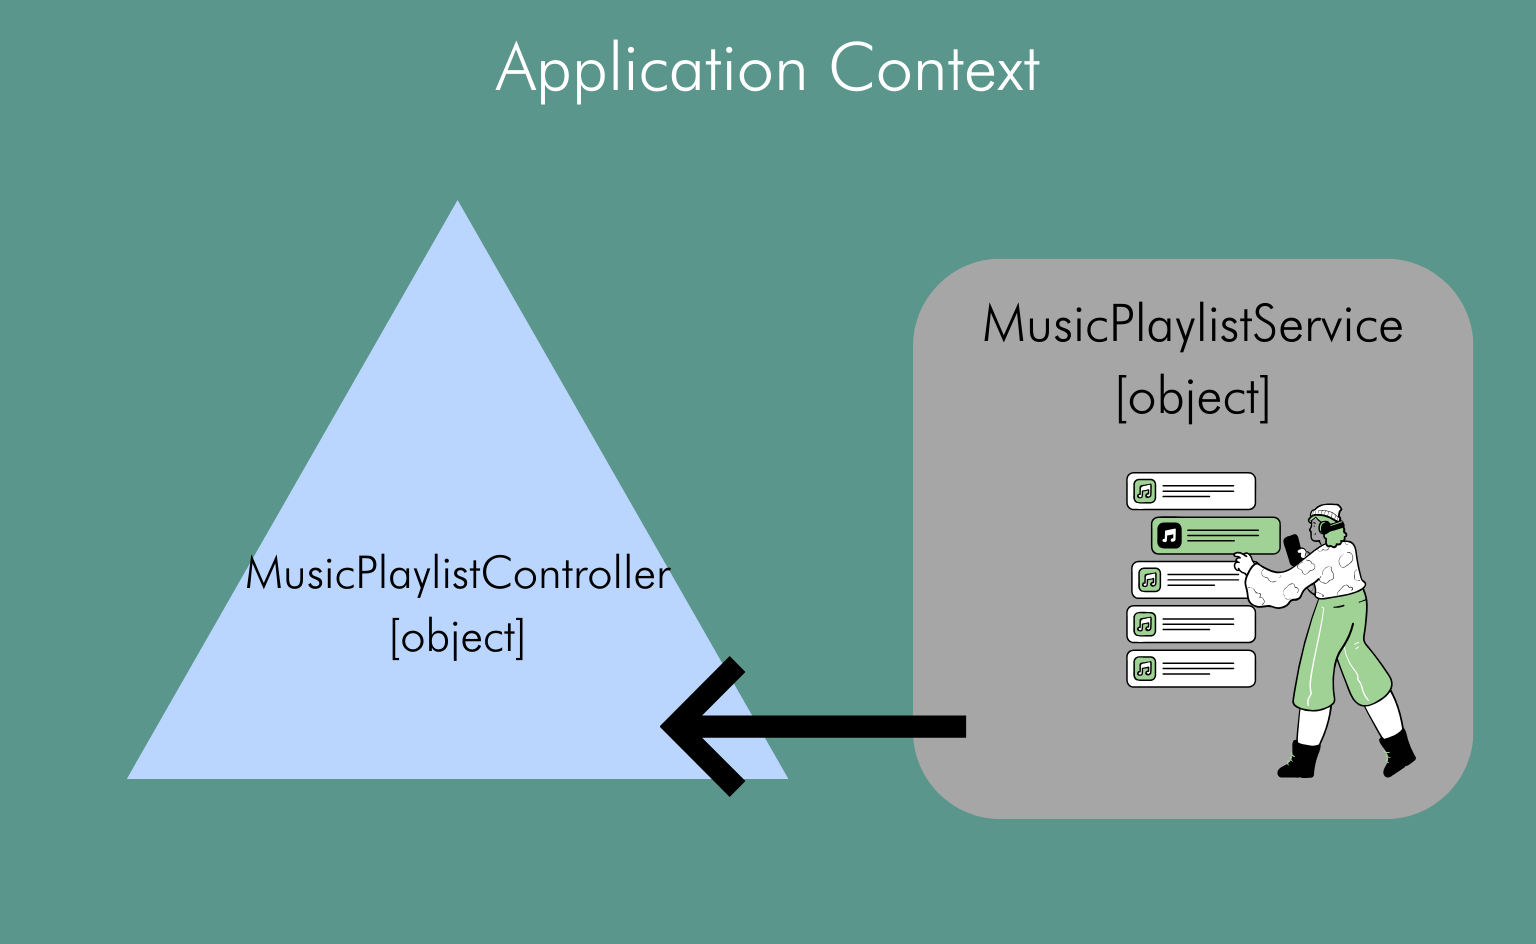
\includegraphics[width=\linewidth]{images/chapter-rest/applicationcontext_musicplaylist.png}
  \caption{Spring Beans in de Application Context}
  \label{fig:spring_beans_musicplaylist}
\end{figure}


\begin{figure}[H]
  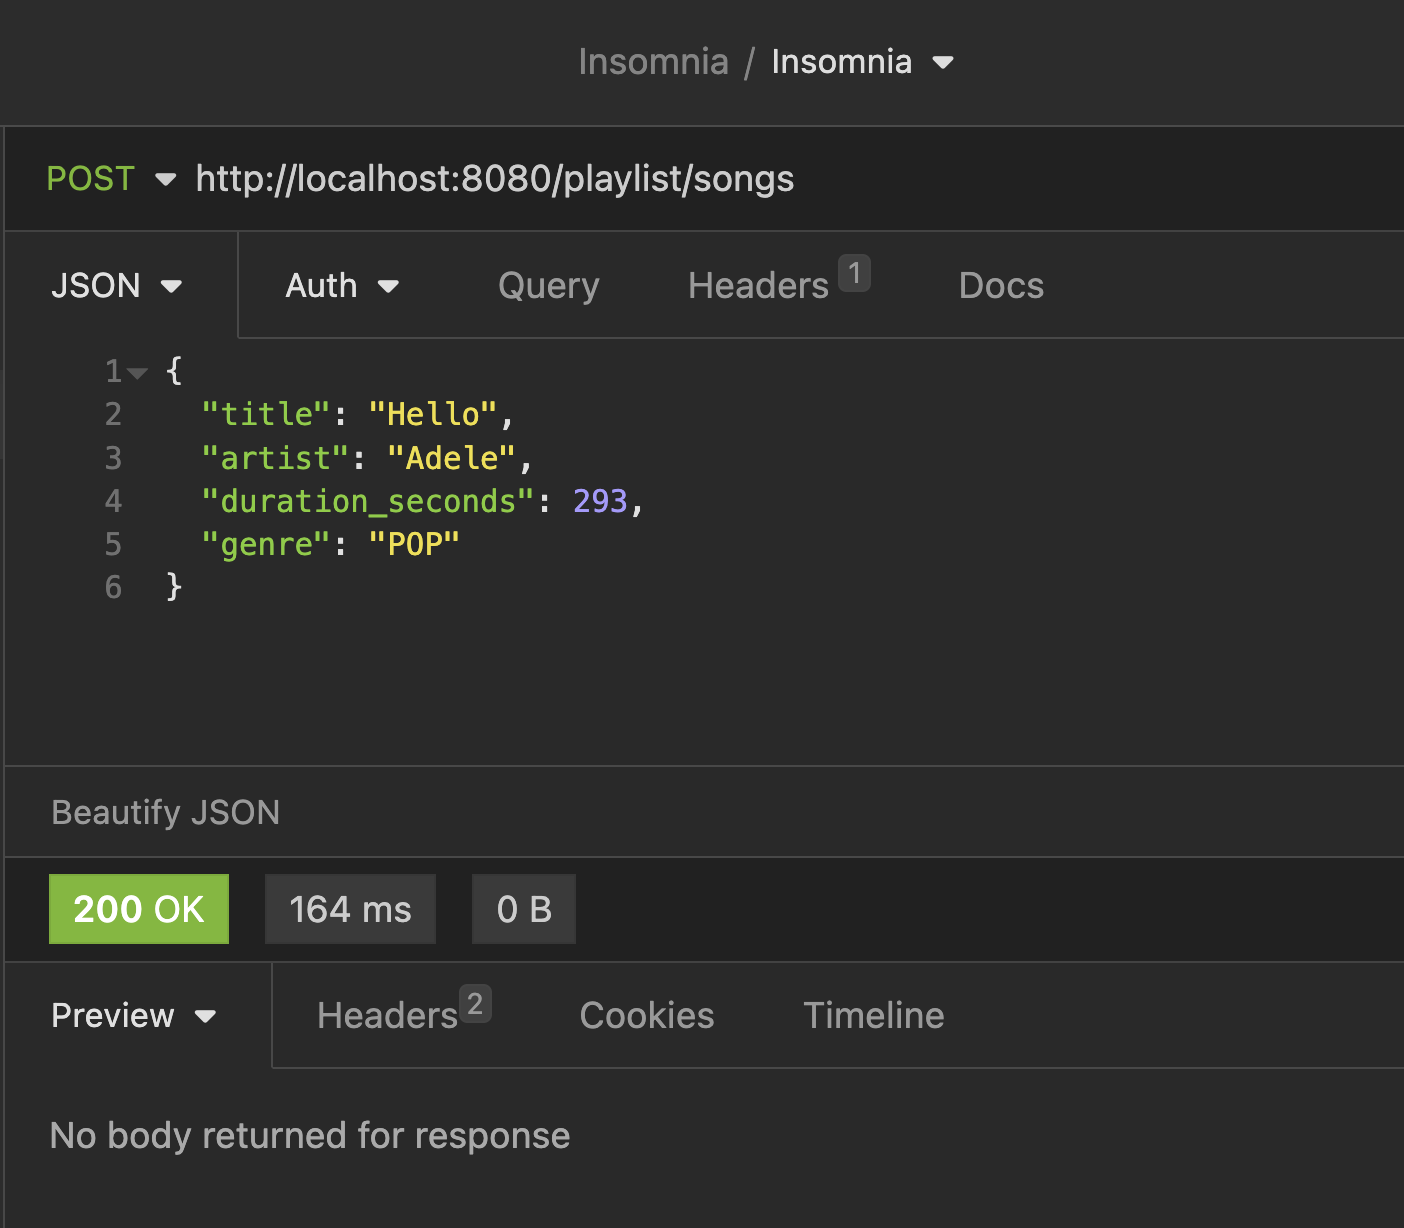
\includegraphics[width=\linewidth]{images/chapter-rest/insomnia_post.png}
  \caption{POST-verzoek met Insomnia}
  \label{fig:post_request}
\end{figure}

\subsection{De playlist opvragen}


\begin{apiRoute}{get}{/playlist/songs}{Retrieve all songs from the playlist}
\begin{routeParameter}
	\noRouteParameter {no parameter }
\end{routeParameter}
\begin{routeRequest}{application/json}
\end{routeRequest}
\begin{routeResponse}{application/json}
\begin{routeResponseItem}{200}{ok}
\begin{routeResponseItemBody}
[
	{
		"title": "Hello",
		"artist": "Adele",
		"genre": "POP",
		"duration_seconds": 293
	},
	{
		"title": "Shape of You",
		"artist": "Ed Sheeran",
		"genre": "POP",
		"duration_seconds": 233
	},
	{
		"title": "Umbrella",
		"artist": "Rihanna",
		"genre": "RNB",
		"duration_seconds": 264
	}
]
\end{routeResponseItemBody}
\end{routeResponseItem}
\end{routeResponse}
\end{apiRoute}


\begin{lstlisting}[language=java,  frame=single]
package be.pxl.demo;

import be.pxl.demo.domain.Song;
import org.springframework.stereotype.Service;

import java.util.ArrayList;
import java.util.List;

@Service
public class MusicPlaylistService {
	private final List<Song> myPlaylist = new ArrayList<>();

	public void addSong(Song song) {
		myPlaylist.add(song);
	}

	public List<Song> getSongs() {
		return myPlaylist;
	}
}
\end{lstlisting}


\begin{lstlisting}[language=java,  frame=single]
package be.pxl.demo.controller;

import be.pxl.demo.MusicPlaylistService;
import be.pxl.demo.domain.Song;
import org.slf4j.Logger;
import org.slf4j.LoggerFactory;
import org.springframework.beans.factory.annotation.Autowired;
import org.springframework.web.bind.annotation.GetMapping;
import org.springframework.web.bind.annotation.PostMapping;
import org.springframework.web.bind.annotation.RequestBody;
import org.springframework.web.bind.annotation.RequestMapping;
import org.springframework.web.bind.annotation.RestController;

import java.util.List;

@RestController
@RequestMapping("/playlist/songs")
public class MusicPlaylistController {

	private static final Logger LOGGER = LoggerFactory.getLogger(MusicPlaylistController.class);
	private final MusicPlaylistService musicPlaylistService;

	@Autowired
	public MusicPlaylistController(MusicPlaylistService musicPlaylistService) {
		this.musicPlaylistService = musicPlaylistService;
	}

	@PostMapping
	public void addSong(@RequestBody Song song) {
		if (LOGGER.isInfoEnabled()) {
			LOGGER.info("Adding song [" + song.getTitle() + "]");
		}
		musicPlaylistService.addSong(song);
	}

	@GetMapping
	public List<Song> getSongs() {
		return musicPlaylistService.getSongs();
	}
}
\end{lstlisting}

\subsection{Liedjes van \'e\'en genre}


 
 \begin{apiRoute}{get}{/playlist/songs/\{genre\}}{Retrieve all songs from the playlist with the given genre}
\begin{routeParameter}
	\routeParamItem{genre}{the requested genre}
\end{routeParameter}
\begin{routeRequest}{application/json}
\end{routeRequest}
\begin{routeResponse}{application/json}
\begin{routeResponseItem}{200}{ok}
\begin{routeResponseItemBody}
[
	{
		"title": "Hello",
		"artist": "Adele",
		"genre": "POP",
		"duration_seconds": 293
	},
	{
		"title": "Shape of You",
		"artist": "Ed Sheeran",
		"genre": "POP",
		"duration_seconds": 233
	}
]
\end{routeResponseItemBody}
\end{routeResponseItem}
\end{routeResponse}
\end{apiRoute}


\begin{lstlisting}[language=java,  frame=single]
package be.pxl.demo.controller;

import be.pxl.demo.MusicPlaylistService;
import be.pxl.demo.domain.Genre;
import be.pxl.demo.domain.Song;
import org.slf4j.Logger;
import org.slf4j.LoggerFactory;
import org.springframework.beans.factory.annotation.Autowired;
import org.springframework.web.bind.annotation.GetMapping;
import org.springframework.web.bind.annotation.PathVariable;
import org.springframework.web.bind.annotation.PostMapping;
import org.springframework.web.bind.annotation.RequestBody;
import org.springframework.web.bind.annotation.RequestMapping;
import org.springframework.web.bind.annotation.RestController;

import java.util.List;

@RestController
@RequestMapping("/playlist/songs")
public class MusicPlaylistController {

	private static final Logger LOGGER = LoggerFactory.getLogger(MusicPlaylistController.class);
	private final MusicPlaylistService musicPlaylistService;

	@Autowired
	public MusicPlaylistController(MusicPlaylistService musicPlaylistService) {
		this.musicPlaylistService = musicPlaylistService;
	}

	@PostMapping
	public void addSong(@RequestBody Song song) {
		if (LOGGER.isInfoEnabled()) {
			LOGGER.info("Adding song [" + song.getTitle() + "]");
		}
		musicPlaylistService.addSong(song);
	}

	@GetMapping
	public List<Song> getSongs() {
		return musicPlaylistService.getSongs();
	}

	@GetMapping("{genre}")
	public List<Song> getSongs(@PathVariable Genre genre) {
		return musicPlaylistService.getSongsByGenre(genre);
	}
}
\end{lstlisting}

\begin{lstlisting}[language=java,  frame=single]
package be.pxl.demo;

import be.pxl.demo.domain.Genre;
import be.pxl.demo.domain.Song;
import org.springframework.stereotype.Service;

import java.util.ArrayList;
import java.util.List;

@Service
public class MusicPlaylistService {
	private final List<Song> myPlaylist = new ArrayList<>();

	public void addSong(Song song) {
		myPlaylist.add(song);
	}

	public List<Song> getSongs() {
		return myPlaylist;
	}

	public List<Song> getSongsByGenre(Genre genre) {
		List<Song> response = new ArrayList<>();
		for (Song song : myPlaylist) {
			if (song.getGenre() == genre) {
				response.add(song);
			}
		}
		return response;
	}
}
\end{lstlisting}


\subsection{Gegevens van een liedje aanpassen}

Als je een nieuwe song in de playlist toevoegt, dan wordt deze steeds achteraan in de lijst toegevoegd. We kunnen nu de gegevens van het liedje op een gegeven positie in de lijst gaan overschrijven of aanpassen.  De index die we meegeven is een waarde van 0 tot 1 minder dan de lengte van de lijst.  Later zullen we zien hoe we een duidelijke foutboodschap kunnen geven aan de client als een foutieve index-waarde wordt gegeven.

Om de gegevens van een liedje aan te passen gebruiken we een PUT-verzoek. 
Je moet steeds alle gegevens van het liedje meegeven in de requestbody. 

\begin{apiRoute}{put}{/musicplaylist/songs\{index\}}{Update the song at the given index.}
\begin{routeParameter}
\routeParamItem{code}{unique identification of a house}
\end{routeParameter}
\begin{routeRequest}{application/json}
\begin{routeRequestBody}
{
		"title": "Hello",
		"artist": "Adele",
		"genre": "POP",
		"duration_seconds": 293
}
\end{routeRequestBody}
\end{routeRequest}
\begin{routeResponse}{application/json}
\begin{routeResponseItem}{200}{ok}
\end{routeResponseItem}
\end{routeResponse}
\end{apiRoute}


\begin{lstlisting}
package be.pxl.demo.controller;

import be.pxl.demo.MusicPlaylistService;
import be.pxl.demo.domain.Genre;
import be.pxl.demo.domain.Song;
import org.slf4j.Logger;
import org.slf4j.LoggerFactory;
import org.springframework.beans.factory.annotation.Autowired;
import org.springframework.web.bind.annotation.DeleteMapping;
import org.springframework.web.bind.annotation.GetMapping;
import org.springframework.web.bind.annotation.PathVariable;
import org.springframework.web.bind.annotation.PostMapping;
import org.springframework.web.bind.annotation.PutMapping;
import org.springframework.web.bind.annotation.RequestBody;
import org.springframework.web.bind.annotation.RequestMapping;
import org.springframework.web.bind.annotation.RestController;

import java.util.List;

@RestController
@RequestMapping("/playlist/songs")
public class MusicPlaylistController {

	private static final Logger LOGGER = LoggerFactory.getLogger(MusicPlaylistController.class);
	private final MusicPlaylistService musicPlaylistService;

	@Autowired
	public MusicPlaylistController(MusicPlaylistService musicPlaylistService) {
		this.musicPlaylistService = musicPlaylistService;
	}

	@PostMapping
	public void addSong(@RequestBody Song song) {
		if (LOGGER.isInfoEnabled()) {
			LOGGER.info("Adding song [" + song.getTitle() + "]");
		}
		musicPlaylistService.addSong(song);
	}

	@GetMapping
	public List<Song> getSongs() {
		return musicPlaylistService.getSongs();
	}

	@GetMapping("/{genre}")
	public List<Song> getSongs(@PathVariable Genre genre) {
		return musicPlaylistService.getSongsByGenre(genre);
	}

	@PutMapping("/{index}")
	public void updateSong(@PathVariable int index, @RequestBody Song song) {
		musicPlaylistService.updateSong(index, song);
	}
}
\end{lstlisting}

\begin{lstlisting}
package be.pxl.demo;

import be.pxl.demo.domain.Genre;
import be.pxl.demo.domain.Song;
import org.springframework.stereotype.Service;

import java.util.ArrayList;
import java.util.List;

@Service
public class MusicPlaylistService {
	private final List<Song> myPlaylist = new ArrayList<>();

	public void addSong(Song song) {
		myPlaylist.add(song);
	}

	public List<Song> getSongs() {
		return myPlaylist;
	}

	public List<Song> getSongsByGenre(Genre genre) {
		List<Song> response = new ArrayList<>();
		for (Song song : myPlaylist) {
			if (song.getGenre() == genre) {
				response.add(song);
			}
		}
		return response;
	}

	public void updateSong(int index, Song song) {
		myPlaylist.set(index, song);
	}

	public void deleteSong(int index) {
		myPlaylist.remove(index);
	}
}
\end{lstlisting}

We vervangen het liedje op de opgegeven index door een nieuw Song-object met de aangepaste gegevens.

\subsection{Een liedje verwijderen}

Om een liedje op een opgegeven index uit de playlist te verwijderen gaan we een DELETE-verzoek implementeren.


\begin{apiRoute}{delete}{/musicplaylist/songs/\{index\}}{Delete the song at the given index.}
\begin{routeParameter}
\routeParamItem{index}{position of the song to be deleted}
\end{routeParameter}
\begin{routeResponse}{application/json}
\begin{routeResponseItem}{200}{ok}
\end{routeResponseItem}
\end{routeResponse}
\end{apiRoute}

\begin{lstlisting}
package be.pxl.demo.controller;

import be.pxl.demo.MusicPlaylistService;
import be.pxl.demo.domain.Genre;
import be.pxl.demo.domain.Song;
import org.slf4j.Logger;
import org.slf4j.LoggerFactory;
import org.springframework.beans.factory.annotation.Autowired;
import org.springframework.web.bind.annotation.DeleteMapping;
import org.springframework.web.bind.annotation.GetMapping;
import org.springframework.web.bind.annotation.PathVariable;
import org.springframework.web.bind.annotation.PostMapping;
import org.springframework.web.bind.annotation.PutMapping;
import org.springframework.web.bind.annotation.RequestBody;
import org.springframework.web.bind.annotation.RequestMapping;
import org.springframework.web.bind.annotation.RestController;

import java.util.List;

@RestController
@RequestMapping("/playlist/songs")
public class MusicPlaylistController {

	private static final Logger LOGGER = LoggerFactory.getLogger(MusicPlaylistController.class);
	private final MusicPlaylistService musicPlaylistService;

	@Autowired
	public MusicPlaylistController(MusicPlaylistService musicPlaylistService) {
		this.musicPlaylistService = musicPlaylistService;
	}

	@PostMapping
	public void addSong(@RequestBody Song song) {
		if (LOGGER.isInfoEnabled()) {
			LOGGER.info("Adding song [" + song.getTitle() + "]");
		}
		musicPlaylistService.addSong(song);
	}

	@GetMapping
	public List<Song> getSongs() {
		return musicPlaylistService.getSongs();
	}

	@GetMapping("/{genre}")
	public List<Song> getSongs(@PathVariable Genre genre) {
		return musicPlaylistService.getSongsByGenre(genre);
	}

	@PutMapping("/{index}")
	public void updateSong(@PathVariable int index, @RequestBody Song song) {
		musicPlaylistService.updateSong(index, song);
	}

	@DeleteMapping("/{index}")
	public void updateSong(@PathVariable int index) {
		musicPlaylistService.deleteSong(index);
	}
}
\end{lstlisting}


\begin{lstlisting}
package be.pxl.demo;

import be.pxl.demo.domain.Genre;
import be.pxl.demo.domain.Song;
import org.springframework.stereotype.Service;

import java.util.ArrayList;
import java.util.List;

@Service
public class MusicPlaylistService {
	private final List<Song> myPlaylist = new ArrayList<>();

	public void addSong(Song song) {
		myPlaylist.add(song);
	}

	public List<Song> getSongs() {
		return myPlaylist;
	}

	public List<Song> getSongsByGenre(Genre genre) {
		List<Song> response = new ArrayList<>();
		for (Song song : myPlaylist) {
			if (song.getGenre() == genre) {
				response.add(song);
			}
		}
		return response;
	}

	public void updateSong(int index, Song song) {
		myPlaylist.set(index, song);
	}

	public void deleteSong(int index) {
		myPlaylist.remove(index);
	}
}
\end{lstlisting}


\begin{oefening}\textbf{Huizenjacht}
We maken een Spring Boot toepassing om het aanbod op de huizenmarkt te beheren.
Ontwikkel een RESTful web toepassing met onderstaande endpoints.
Je voorziet een component HouseService met \'e\'en enkele, gedeelde lijst van woningen  voor alle gebruikers.

Een huis wordt voorgesteld als een resource met volgende eigenschappen:

\begin{itemize}
  \item \texttt{code} (string): Unieke identificatie van het huis.
  \item \texttt{name} (string): Naam of beschrijving van het huis.
  \item \texttt{status} (enum): Status FOR\_SALE of SOLD.
  \item \texttt{city} (string): Locatie van het huis.
  \item \texttt{price} (double): Prijs van het huis.
\end{itemize}

\section{REST Endpoints}

\begin{apiRoute}{post}{/houses}{Create a new house.}
\begin{routeParameter}
	\noRouteParameter {no parameter }
\end{routeParameter}
\begin{routeRequest}{application/json}
\begin{routeRequestBody}
{
  "code": "HAS_001",
  "name": "Beautiful house in the city",
  "city": "Hasselt",
  "price": 250000
}
\end{routeRequestBody}
\end{routeRequest}
\begin{routeResponse}{application/json}
\begin{routeResponseItem}{200}{ok}
\end{routeResponseItem}
\end{routeResponse}
\end{apiRoute}


\begin{apiRoute}{put}{/houses/\{code\}}{Update the data (status, price,...) of the house with the given code.}
\begin{routeParameter}
\routeParamItem{code}{unique identification of a house}
\end{routeParameter}
\begin{routeRequest}{application/json}
\begin{routeRequestBody}
{
  "status": "SOLD"
  "name": "Beautiful house in the city",
  "price": 320000
}
\end{routeRequestBody}
\end{routeRequest}
\begin{routeResponse}{application/json}
\begin{routeResponseItem}{200}{ok}
\end{routeResponseItem}
\end{routeResponse}
\end{apiRoute}

\begin{apiRoute}{get}{/houses}{Retrieve all houses.}
\begin{routeParameter}
	\noRouteParameter {no parameter }
\end{routeParameter}
\begin{routeResponse}{application/json}
\begin{routeResponseItem}{200}{ok}
\begin{routeResponseItemBody}
[
  {
    "code": "GNK_001",
    "name": "Beautiful house in the city",
    "status": "SOLD",
     "city": "Genk",
    "price": 250000
  },
  {
    "code": "HAS_003",
    "name": "Cozy bungalow",
    "status": "FOR_SALE",
     "city": "Hasselt",
    "price": 180000
  }
]
\end{routeResponseItemBody}
\end{routeResponseItem}
\end{routeResponse}
\end{apiRoute}

\begin{apiRoute}{delete}{/houses/\{code\}}{Delete the house with the given code.}
\begin{routeParameter}
\routeParamItem{code}{unique identification of a house}
\end{routeParameter}
\begin{routeResponse}{application/json}
\begin{routeResponseItem}{200}{ok}
\end{routeResponseItem}
\end{routeResponse}
\end{apiRoute}

\end{oefening}

\chapter{Unit testing}

\begin{summary}
De software die we ontwikkelen moet kwaliteitsvol zijn. Maar hoe kunnen we er nu voor zorgen dat we het aantal bugs in onze code zo laag mogelijk houden? E\'en van de strategie\"en om de kwaliteit van software te waarborgen is testen. Testen is een heel belangrijk aspect van softwareontwikkeling waar je ongetwijfeld nog heel veel over gaat leren. 

Als ontwikkelaar zorg je er altijd voor dat wanneer je de gevraagde functionalteit implementeert, je ook de nodige unit testen schrijft om de kwaliteit van je code te garanderen. Wanneer je unit testen schrijft, ga je alle methoden van je klasse testen. Een methode van een klasse is dus de ``unit'' die we gaan testen.
We gaan automatische testen schrijven. Dit betekent dat iedere keer dat de code wordt aangepast of uitgebreid de testen eenvoudig opnieuw kunnen worden uitgevoerd. Op die manier gaan de fouten die ontstaan tijdens de verdere ontwikkeling van de software snel ontdekt worden. Bedenk ook dat een fout, onduidelijkheid of bug die vroeg in het ontwikkelproces wordt aangepakt, maar een kleine impact heeft (ook financieel) ten opzicht van problemen die later pas opduiken.
\end{summary}

\section{JUnit}

In Java gaan we gebruikmaken van het framework JUnit5 om onze unit testen te schrijven.
JUnit5 is opgedeeld in 3 sub-projecten:  Jupiter, Vintage en Platform. JUnit Jupiter is het  sub-project dat wij gebruiken om onze testen te schrijven en voorziet de engine om deze testen uit te voeren.


https://education.launchcode.org/java-web-development/chapters/unit-testing/exercises.html

https://www.didattica.agentgroup.unimo.it/wiki/images/7/7b/Es01-JUnit.pdf

\section{Unit test voor een constructor}

We starten direct met een voorbeeld. In het vorige hoofdstuk hadden we de klasse Documentary aangemaakt. De klasse Documentary is een subklasse van Movie. Bij het aanmaken van een Documentary-object moet wel steeds als genre Genre.DOCUMENTARY ingevuld zijn. 

\begin{lstlisting}
package be.pxl.ja.opdracht1;

public class Documentary extends Movie {

	private String topic;

	public Documentary(String title, Rating rating) {
		super(title, rating);
		addGenre(Genre.DOCUMENTARY);
	}

	public String getTopic() {
		return topic;
	}

	public void setTopic(String topic) {
		this.topic = topic;
	}
}
\end{lstlisting}

We gaan dus de constructor van de klasse Documentary testen.

Onze testklassen gaan we niet mengen met onze eigenlijke programma. Ons hoofdprogramma en de klassen zitten meestal in een source-folder (src). Onze unit testen plaatsen we in een overeenkomstig package in de test-folder. Wanneer je een folder met de naam ``test'' hebt aangemaakt, markeer deze dan ook als test-folder.


\begin{lstlisting}
package be.pxl.ja.opdracht1;

import org.junit.jupiter.api.Test;

import static org.junit.jupiter.api.Assertions.assertEquals;

public class DocumentaryTest {

	private static final String TITLE = "Planet Earth";

	@Test
	public void documentaryConstructor() {
		// ACT
		Documentary documentary = new Documentary(TITLE, Rating.TEENS);

		// ASSERT
		assertEquals(TITLE, documentary.getTitle());
		assertEquals(Rating.TEENS, documentary.getRating());
		assertEquals(Genre.DOCUMENTARY, documentary.getGenre());
	}
}
\end{lstlisting}

\global\csname @topnum\endcsname 0

We hoeven enkel een @Test annotatie toe te voegen opdat een test herkend wordt en uitgevoerd kan worden. De eerste keer dat je de annotatie @Test toevoegt in het project zal deze nog niet gekend zijn. IntelliJ zal zelf voorstellen om JUnit te downloaden en toe te voegen aan het classpath. Zorg er wel voor dat je de juiste versie gebruikt. 


Wanneer je nu de unit test DocumentaryTest uitvoert kunnen er 3 mogelijke scenario's plaatsvinden. Ofwel slaagt de test, ofwel faalt \'e\'en van de beweringen (asserts) ofwel loopt er iets onverwachts fout. In het eerste geval krijgt je test een groene kleurcode, in het tweede scenario een oranje en in het laatste scenario een rode.

\begin{figure}[H]
  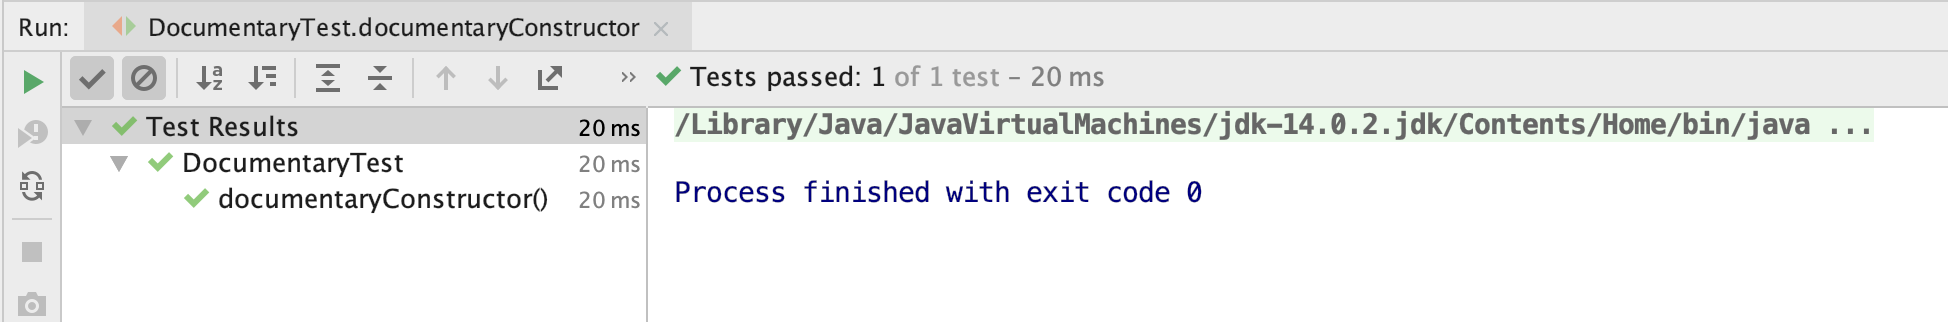
\includegraphics[width=\linewidth]{images/chapter-junit/junit_test_passed.png}
  \caption{Geslaagde JUnit5 test}
  \label{fig:test_passed}
\end{figure}

\begin{figure}[H]
  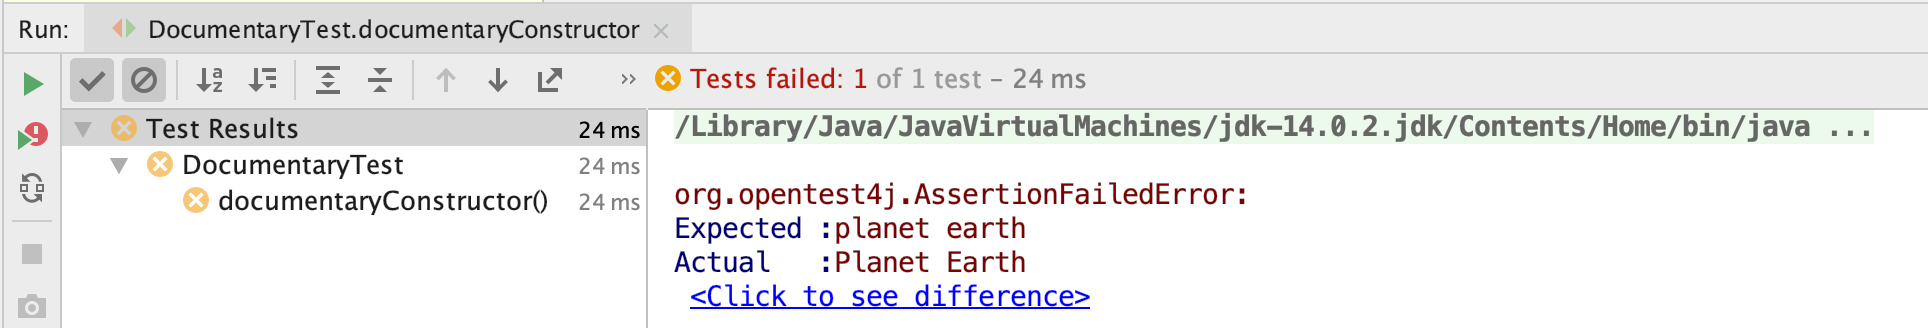
\includegraphics[width=\linewidth]{images/chapter-junit/junit_test_failed.png}
  \caption{Gefaalde JUnit5 test}
  \label{fig:test_failed}
\end{figure}



De methode van de Nederlandse weeramateurs is simpel. Het weercijfer tussen 0 en 10 wordt bepaald uit het weer overdag, tussen 7 en 19 uur. Een droge dag met nauwelijks bewolking of mist en weinig wind krijgt een 10. Afhankelijk van de hoeveelheid wolken vermindert dit met 1 tot 3 punten. Is het mistig dan kost dat, afhankelijk van de duur 1 of 2 punten. Voor de regen telt het aantal uurvakken met neerslag, dus ook alleen de duur. Zijn er tussen 7 en 19 uur twee uurvakken met regen dan kost dat 1 punt. Maar regent het in 11 of 12 uurvakken dan kost dat 4 punten.

Een zwakke wind kost geen punten, maar een matige wind van windkracht 3 gedurende minstens 3 uur kost 1 punt. De temperatuur speelt geen rol, zodat het weercijfer objectief is en ook koude, mooie dagen gunstig scoren. Langdurige regen overdag en veel wind leveren altijd een lage score.

\section{Unit test voor een setter}

Onze test zal steeds opgebouwd worden volgens het 3A patroon: Arrange, Act en Assert.
In iedere test herken je steeds deze 3 bouwstenen. 

Het ``arrange''-gedeelte is waar het object dat getest moet worden en alle andere objecten - die nodig zijn om de test goed uit te voeren - worden aangemaakt. 
Het ``act''-gedeelte is waar we de methode die we willen testen aanroepen. Als de methode een returnwaarde heeft ken je dit toe aan een variabele.

Het ``assert''-gedeelte geeft je de mogelijkheid om beweringen over het resultaat te verifi\"eren.

Hier is nog eens de klasse Movie.

\begin{lstlisting}
import java.time.LocalDate;

public class Movie extends Content implements Playable {
	private String director;
	private LocalDate releaseDate;
	private int duration;

	public Movie(String title, Rating rating) {
		super(title, rating);
	}

	public String getDirector() {
		return director;
	}

	public void setDirector(String director) {
		this.director = director;
	}

	public LocalDate getReleaseDate() {
		return releaseDate;
	}

	public void setReleaseDate(LocalDate releaseDate) {
		this.releaseDate = releaseDate;
	}

	public int getDuration() {
		return duration;
	}

	@Override
	public void play() {
		System.out.println("Playing " + this);
	}

	@Override
	public void pause() {
		System.out.println("Pausing " + this);
	}

	public boolean isLongPlayingTime() {
		return duration > LONG_PLAYING_TIME;
	}

	public String getPlayingTime() {
		// TODO: implement this method correctly		
		return "2 u 30 min";
	}

	@Override
	public String toString() {
		StringBuilder builder = new StringBuilder(super.toString());
		if (releaseDate != null) {
			builder.append(" (").append(releaseDate.getYear()).append(")");
		}
		return builder.toString();
	}
}
\end{lstlisting}

\global\csname @topnum\endcsname 0

Bekijk de methode void setDuration(int duration) eens. We willen nooit een negatief getal als waarde voor de eigenschap duration. Daarom zullen we de absolute waarde nemen van de parameter duration. Om deze setter te testen gaan we 2 testen voorzien. Een eerste test waar we een positieve waarde meegeven als argument en een tweede test waarbij we een negatieve waarde meegeven.

\begin{lstlisting}
import org.junit.jupiter.api.Test;

import static org.junit.jupiter.api.Assertions.assertEquals;

public class MovieSetDurationTest {

	@Test
	public void negativeDurationBecomesPositive() {
		// ARRANGE
		Movie movie = new Movie("Titanic", Rating.OLDER_KIDS);

		// ACT
		movie.setDuration(-125);

		// ASSERT
		assertEquals(125, movie.getDuration());
	}

	@Test
	public void positiveDurationStaysUnchanged() {
		// ARRANGE
		Movie movie = new Movie("Titanic", Rating.OLDER_KIDS);

		// ACT
		movie.setDuration(125);

		// ASSERT
		assertEquals(125, movie.getDuration());
	}
}
\end{lstlisting}

\clearpage

\section{Unit test voor een getter}

In de klasse Movie vind je ook de methode isLongPlayingTime() terug. Deze methode heeft een boolean als resultaat-type en geeft true indien de film langer dan 2 u 15 min duurt.

Hier is alvast 1 mogelijke unit test.

\begin{lstlisting}
import static org.junit.jupiter.api.Assertions.assertFalse;

public class MovieIsLongPlayingTimeTest {
	
	@Test
	public void movieWithDurationShorterThanLongPlayingTimeReturnsFalse() {
		
		Movie movie = new Movie("Titanic", Rating.TEENS);
		
		movie.setDuration(Movie.LONG_PLAYING_TIME - 1);
		
		assertFalse(movie.isLongPlayingTime());
	}
}
\end{lstlisting}

Bij de overige testen zullen in het Arrange gedeelte opnieuw een Movie-object moeten aanmaken. Omdat dit voor iedere test herzelfde is, hoeven we deze code niet te dupliceren. 
Met de annotatie @BeforeEach kunnen we een methode aanduiden die wordt uitgevoerd voor elke test.

Daarnaast merk je ook dat de klasse org.junit.jupiter.api.Assertions bijkomende static methoden heeft om de resultaten van de test te verifi\"eren. \textbf{assertFalse} en \textbf{assertTrue} zullen  slagen als de getestte waarde repectievelijk false of true is.

\begin{lstlisting}
import org.junit.jupiter.api.BeforeEach;
import org.junit.jupiter.api.Test;

import static org.junit.jupiter.api.Assertions.assertFalse;
import static org.junit.jupiter.api.Assertions.assertTrue;

public class MovieIsLongPlayingTimeTest {

	private Movie movie;

	@BeforeEach
	public void init() {
		movie = new Movie("Titanic", Rating.TEENS);
	}

	@Test
	public void movieWithDurationShorterThanLongPlayingTimeReturnsFalse() {

		movie.setDuration(Movie.LONG_PLAYING_TIME - 1);

		assertFalse(movie.isLongPlayingTime());
	}

	@Test
	public void movieWithDurationExactlyLongPlayingTimeReturnsFalse() {

		movie.setDuration(Movie.LONG_PLAYING_TIME);

		assertFalse(movie.isLongPlayingTime());
	}

	@Test
	public void movieWithDurationLongerThanLongPlayingTimeReturnsTrue() {

		movie.setDuration(Movie.LONG_PLAYING_TIME + 1);

		assertTrue(movie.isLongPlayingTime());
	}
}
\end{lstlisting}

We maken ook in de testen handig gebruik van de constante LONG\_PLAYING\_TIME. Door onze testen op deze manier te schrijven hoeven we de testen niet aan te passen als de waarde van LONG\_PLAYING\_TIME wordt aangepast. 

Hier is een overzicht van enkele handige static methoden uit de klasse org.junit.jupiter.api.Assertions. 

\begin{table}[h!]
\centering
\begin{tabularx}{\textwidth}{| l | X |}
 \hline
 Methode & Betekenis\\ 
 \hline\hline
assertEquals() & Evalueert de gelijkheid van 2 waarden. De test slaagt als beide
waarden gelijk (equal) zijn.\\
\hline
assertFalse() & Evaluatie van een booleaanse uitdrukking. De test slaagt indien
de uitdrukking false is.\\
\hline
assertTrue() & Evaluatie van een booleaanse uitdrukking. De test slaagt indien
de uitdrukking true is.\\
\hline
assertNotNull( ) & Vergelijkt een object referentie met null. De test slaagt indien de
object referentie niet null is.\\
\hline
assertSame( ) & Vergelijkt het geheugenadres van twee object referenties
(gebruik maken van == operator). De test slaagt indien beide
object referenties naar hetzelfde object verwijzen.\\
\hline
fail() & Zorgt ervoor dat de test zal falen.\\
 \hline
\end{tabularx}
\caption{Static methoden uit de klasse org.junit.jupiter.api.Assertions}
\label{table:assertions}
\end{table}

\begin{oefening}
Schrijf 2 unit testen voor de toString() methode van de klasse Movie. We verwachten dat deze methode de titel en het jaartal van de film teruggeeft (bijv. Titanic (1997)). Indien er geen releasedatum gekend is, wordt het jaartal achterwege gelaten.
\end{oefening}

\begin{oefening}
Schrijf unit testen voor de methode addGenre in de klasse Content. Let er ook op dat een  genre enkel wordt toegevoegd indien het niet eerder al werd toegevoegd. 
\end{oefening}

\begin{oefening}
Je ziet dat in bovenstaande klasse Movie de methode getPlayingTime() nog niet correct ge\"implementeerd is. Hier zijn alvast de unit testen. 

\begin{lstlisting}
import org.junit.jupiter.api.BeforeEach;
import org.junit.jupiter.api.Test;

import static org.junit.jupiter.api.Assertions.assertEquals;

public class MovieGetPlayingTimeTest {

	private Movie movie;

	@BeforeEach
	public void init() {
		movie = new Movie("Titanic", Rating.OLDER_KIDS);
	}

	@Test
	public void returnsQuestionmarkWhenDurationZero() {

		movie.setDuration(0);

		assertEquals("?", movie.getPlayingTime());
	}

	@Test
	public void returnsMinutesWhenDurationLessThan60() {

		movie.setDuration(59);

		assertEquals("59 min", movie.getPlayingTime());
	}

	@Test
	public void returnsHoursWhenDurationMultipleOf60() {

		movie.setDuration(120);

		assertEquals("2 h", movie.getPlayingTime());
	}

	@Test
	public void returnsHoursAndMinutesWhenDurationNotMultipleOf60() {

		movie.setDuration(135);

		assertEquals("2 h 15 min", movie.getPlayingTime());
	}
}
\end{lstlisting}

Bestudeer deze unit testen en implementeer vervolgens de methode. Test je implementatie uit! Wanneer alle testen slagen, bekijk dan je je code nog eens kritisch. Kan je nog verbeteringen aanbrengen in de code?
\end{oefening}

Je ziet dat je geen schrik moet hebben om achteraf je code te verbeteren. Omdat je beschikt over unit testen kan je rustig aan je code gaan sleutelen. Het proces om code te verbeteren en hierdoor de leesbaarheid en onderhoudbaarheid van de code te verhogen noemen we \textbf{refactoren}. 

\begin{remark}
  Meer weten over unit testing, kijk op pluralsight: \url{https://app.pluralsight.com/library/courses/junit-5-unit-testing-getting-started}
\end{remark}

\begin{oefening}
We gaan bij de domeinklassen van de streaming service nog enkele klassen en enums toevoegen. Deze klassen gaan we hergebruiken tijdens latere oefeningen. 

Je implementeert volgende enums en klassen in je oplossingen van opgave 1:
\begin{itemize}
\item CreditCardType
\item PaymentInfo
\item StreamingPlan
\item Profile
\item Account
\end{itemize}

\textbf{Enum CreditCardType}

CreditCardType is een eenvoudige enum-klasse met de waarden VISA en MASTERCARD.

\textbf{Klasse PaymentInfo}

Wanneer een gebruiker een account aanmaakt voor onze streaming service moet hij zijn betaalgegevens opgegeven. Deze gegevens houden we bij in een PaymentInfo-object.
Deze klasse bevat de volgende eigenschappen:

\begin{itemize}
\item cardNumber (String)
\item type (CreditCardType)
\item firstName (String)
\item lastName (String)
\item expirationDate (LocalDate)
\item securityCode (int)
\end{itemize}

Je hoeft enkel getters en setters te voorzien. Het valideren van cardNumber, securityCode en expirationDate houden we voor het volgende hoofdstuk wanneer we het hebben over foutafhandeling.

\textbf{Enum StreamingPlan}

Er zijn 3 producten waaruit gebruikers kunnen kiezen. Ieder product heeft een maximum aantal profielen per account en een prijs. 

Gebruikers met product BASIC kunnen maar 1 profiel aanmaken en betalen €7,99.
Gebruikers die kiezen voor STANDAARD kunnen 2 profielen aanmaken en betalen €11,99.
Tenslotte kunnen gebruikers met een PREMIUM account 4 profielen aanmaken. Zij betalen €15,99.

Maak een enum met de naam StreamingPlan met deze producten. Gebruik numberOfProfiles en price als eigenschappen voor deze enum-klasse. 

\textbf{Klasse Profile}

Afhankelijk van de StreamingPlan kunnen er dus profielen toegevoegd worden aan een account. Daarom implementeren we de klasse Profile. Voor iedere Profile-object willen we een naam (name) en een geboortedatum (dateOfBirth) weten. Deze laatste hebben we nodig om te beslissen of Content beschikbaar is of niet. 

Hiervoor voorzie je een methode \textit{boolean allowedToWatch(Content content)} in de klasse Profile. De methode geeft true als de content geschikt is voor het profiel (afhankelijk van de rating van de content en de geboortedatum van het profiel). 
De methode geeft false als de content niet geschikt is voor het profiel.
Zolang de geboortedatum niet is ingevuld is alle content niet geschikt voor het profiel.
Voeg de nodige unit testen toe om deze methode grondig te testen!

\textbf{Klasse Account}

En tenslotte voeg je de klasse Account toe. Een account heeft volgende eigenschappen:
\begin{itemize}
\item email
\item password
\item streamingPlan
\item \'e\'en of meerder profielen
\item paymentInfo
\end{itemize}

In de constructor van een Account wordt er direct 1 profiel aangemaakt met de naam "profile1" en geboortedatum 1/1/2000. Schrijf unit testen voor de constructor.

De methode getFirstProfile() geeft het eerste (en voorlopig ook enige) Profile-object terug als resultaat. 

De functionaliteit om profielen toe te voegen wordt in een volgend hoofdstuk toegevoegd.

\textbf{Optioneel: Sterkte van het paswoord}

Wanneer de gebruiker een account aanmaakt kiest hij een paswoord. We geven hem graag een indicatie of zijn gekozen paswoord voldoende sterk is.
Maak een hulpklasse \textbf{PasswordUtil}  met een static methode \textit{int calculateStrength(String password)}. 

Hier zijn de regels voor de berekening van de sterkte van een paswoord:
\begin{itemize}
\item Een paswoord met minder dan 6 karakters is zwak en geeft altijd een score van 0.
\item Een paswoord met een lengte tussen 6 en 10 geeft een score van 1.
\item Een paswoord met meer dan 10 karaketer geeft een score van 2.
\end{itemize}
Voor paswoorden met een lengte vanaf 6 karakters gelden de volgende bijkomende regels:
\begin{itemize}
\item Indien het paswoord minstens 1 cijfer bevat, wordt de score met 2 verhoogd.
\item Indien het paswoord minstens 1 kleine letter bevat, wordt de score met 2 verhoogd.
\item Indien het paswoord minstens 1 hoofdletter bevat, wordt de score met 2 verhoogd.
\item Indien het paswoord minstens 1 special karakter bevat, wordt de score met 2 verhoogd. Er is reeds een constante aanwezig in de klasse PasswordUtil die de speciale karakters bevat.
\end{itemize}
Implementeer deze regels en schrijf de nodige unit testen.
\end{oefening}

TODO klassendiagram



@Service
public class MusicPlaylistService {

    public String calculatePlaylistDuration(List<String> songDurations) {
        int totalSeconds = 0;

        for (String duration : songDurations) {
            String[] parts = duration.split(":");
            if (parts.length == 2) {
                int minutes = Integer.parseInt(parts[0]);
                int seconds = Integer.parseInt(parts[1]);
                totalSeconds += (minutes * 60) + seconds;
            }
        }

        int hours = totalSeconds / 3600;
        int remainingSeconds = totalSeconds % 3600;
        int minutes = remainingSeconds / 60;
        int seconds = remainingSeconds % 60;

        return String.format("%d:%02d:%02d", hours, minutes, seconds);
    }
}


\chapter{Streams}

\begin{summary}
De Stream API van Java biedt een elegante manier om collections te manipuleren. De belangrijkste interface uit de API is Stream$<$T$>$. Als Java ontwikkelaar gebruik je voornamelijk deze interface die alle implementatie-details verbergt. Bij het ontwerpen van de Stream API is, naast het aanbieden van een elegante en eenvoudige API, ook veel aandacht besteed aan performantie. 
\end{summary}

\section{External en internal iterators}

Veronderstel dat we een verzameling met Movie-objecten hebben: \textit{movies}. We willen nu graag weten hoeveel actiefilms er in onze verzameling zitten.

Hier is de code om dit te berekenen.

\begin{lstlisting}
int count = 0;
for (Movie movie: movies) {
    if (movie.getGenre() == Genre.ACTION) {
        count++;
    }
}
\end{lstlisting}

Bovenstaand voorbeeld bevat veel boilerplate code en daarnaast hebben we ook een external iterator. 

Een stream maakt het mogelijk om op een functionele manier complexe bewerkingen uit te voeren op een verzameling.
We kunnen bovenstaande code schrijven met behulp van een stream. Onze external iterator verdwijnt en we krijgen een internal iterator in de plaats.

\begin{lstlisting}
int count = movies.stream().filter(m -> m.getGenre() == Genre.ACTION).count();
\end{lstlisting}

Een stream bestaat uit 3 delen: een (data) bron, intermediate operations (tussentijdse bewerkingen) en een terminal operation (eindbewerking). In ons voorbeeld is de verzameling movies de bron, vervolgens hebben we een intermediate operation \textit{filter} en tenslotte een terminal operation \textit{count}.

\begin{figure}[H]
  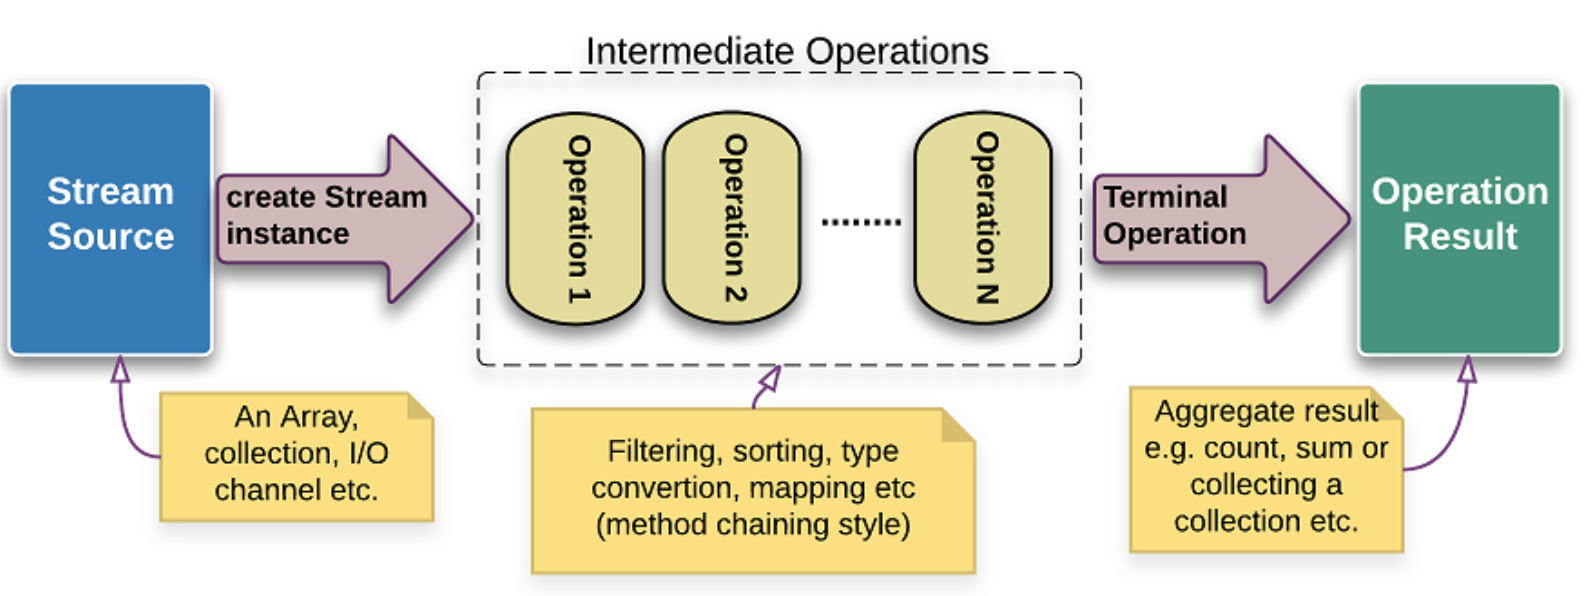
\includegraphics[width=\linewidth]{images/chapter_streams/stream_pipeline.png}
  \caption{Stream pipeline (logicbig.com)}
  \label{fig:stream_of}
\end{figure}


De intermediate operators verwerken de elementen van de stream \'e\'en voor \'e\'en. Alle intermediate operations zijn lui (lazy), ze worden enkel uitgevoerd als de stream wordt afgesloten door een terminal operation.

De internal iterator geniet meestal de voorkeur. Internal iterations kunnen korter geschreven worden en zijn daardoor ook makkelijker lees- en onderhoudbaar. Toch zijn er situaties, zoals wanneer je 2 verzamelingen gelijktijdig manipuleert, dat je kiest voor een external iterator.

\begin{figure}[H]
  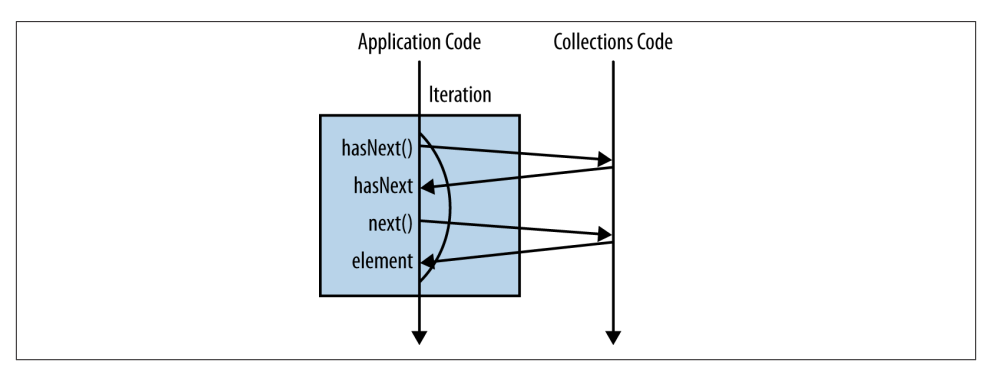
\includegraphics[width=\linewidth]{images/chapter_streams/external_iteration.png}
  \caption{External iteration}
  \label{fig:external_iteration}
\end{figure}

\begin{figure}[H]
  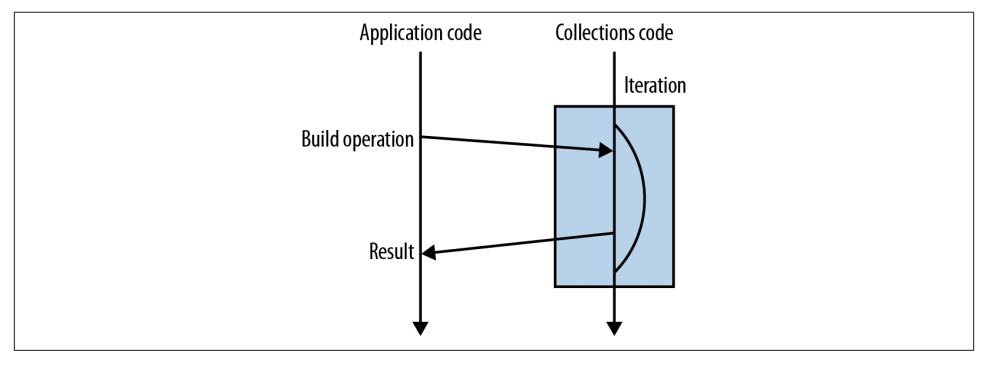
\includegraphics[width=\linewidth]{images/chapter_streams/internal_iteration.png}
  \caption{Internal iteration}
  \label{fig:internal_iteration}
\end{figure}

\section{Intermediate en terminal operations}

\subsection{Terminal operation .collect()}

\begin{lstlisting}
import java.util.List;
import java.util.stream.Collectors;
import java.util.stream.Stream;

public class DemoCollect {

	public static void main(String[] args) {

		List<String> theBeatles = 
				Stream.of("John Lennon", "Paul McCartney", "George Harrison", "Ringo Starr")
				.collect(Collectors.toList());
		System.out.println(theBeatles);
	}

}
\end{lstlisting}

Een stream is geen datastructuur of verzameling. Je moet een stream zien als een reeks objecten. E\'en van de manieren om zo'n reeks of stream te bouwen is met de static methode \textit{of} van de interface Stream.

\begin{figure}[H]
  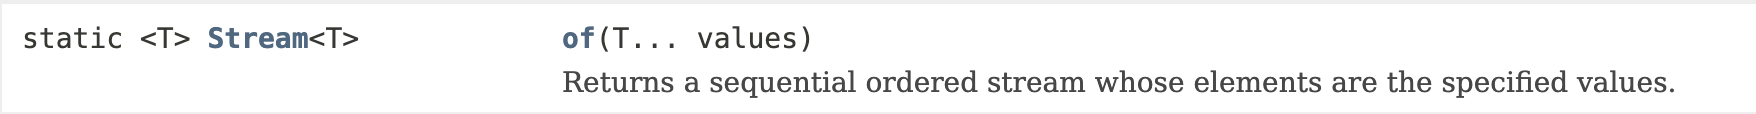
\includegraphics[width=\linewidth]{images/chapter_streams/stream_of.png}
  \caption{Static methode of() in de interface Stream}
  \label{fig:stream_of}
\end{figure}

Door gebruik te maken van de operation \textit{collect(Collectors.toList())} kunnen we de objecten uit de stream verzamelen in een List.

\subsection{Intermediate operation .filter()}

Wanneer je bepaalde elementen uit een stream wil selecteren, gebruik je een filter. 

\begin{figure}[H]
  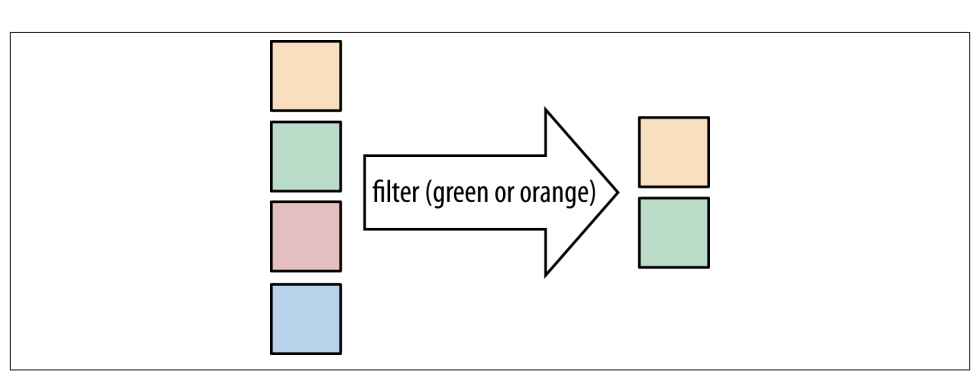
\includegraphics[width=\linewidth]{images/chapter_streams/illustration_filter.png}
  \caption{Filter operation}
  \label{fig:filter_operation}
\end{figure}

\begin{figure}[H]
  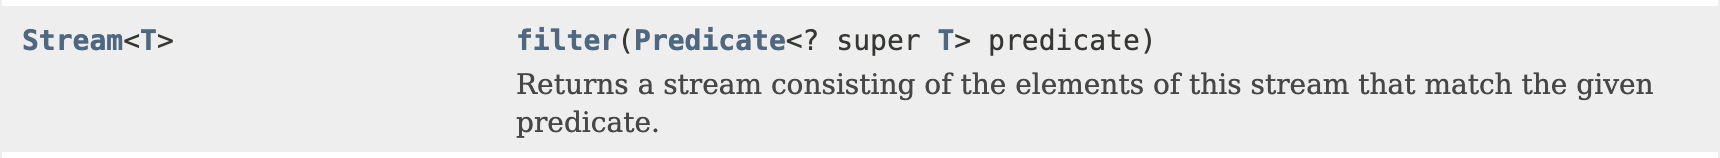
\includegraphics[width=\linewidth]{images/chapter_streams/stream_filter.png}
  \caption{Methode filter() in de interface Stream}
  \label{fig:stream_filters}
\end{figure}

Aan de hand van een Predicate wordt beslist welke elementen geselecteerd worden. 

In het onderstaande voorbeeld selecteren we de even getallen uit de verzameling numbers.

\begin{lstlisting}
List<Integer> numbers = Arrays.asList(1,2,3,4,5);

List<Integer> evenNumbers = numbers.stream()
				.filter(n -> n%2  == 0)
				.collect(Collectors.toList());
				
assertEquals(Arrays.asList(2,4), evenNumbers);
\end{lstlisting}

Nog een voorbeeld.

\begin{lstlisting}
List<String> animals = Stream.of("zebra", "dog", "dolphine")
				.filter(a -> a.contains("o"))
				.collect(Collectors.toList());

assertEquals(Arrays.asList("dog", "dolphine"), animals);
\end{lstlisting}

Alle String-objecten die een ``o'' bevatten mogen in de stream aanwezig blijven.

Merk op dat de functie filter() een intermediate operation is. De bewerking heeft als return-type Stream. We bouwen als het ware een pipeline. De filter()-operation is ook lazy en zal pas effectief uitgevoerd worden als er een terminal-operation aanwezig is.

Hier volgt nog een voorbeeld met een verzameling met objecten van een zelfgeschreven klasse Participant.

\begin{lstlisting}
public class Participant {
	private String name;
	private int points;

	public Participant(String name, int points) {
		this.name = name;
		this.points = points;
	}

	public int getPoints() {
		return points;
	}

	public String getName() {
		return name;
	}
}
\end{lstlisting}

\begin{lstlisting}
Participant john = new Participant("John P.", 15);
Participant sarah = new Participant("Sarah M.", 200);
Participant charles = new Participant("Charles B.", 150);
Participant mary = new Participant("Mary T.", 1);

List<Participant> participants = Arrays.asList(john, sarah, charles, mary);

List<Participant> over100Points = participants.stream()
     .filter(p -> p.getPoints() > 100)
     .collect(Collectors.toList());

assertEquals(Arrays.asList(sarah, charles), over100Points);
\end{lstlisting}

Je kan ook meerdere criteria gebruiken in een filter. Je kan in het Predicate de verschillende criteria samenvoegen via boolean operatoren.

\begin{lstlisting}
List<Participant> selection = participants.stream()
    .filter(p -> p.getPoints() > 100 && p.getName().startsWith("S"))
    .collect(Collectors.toList());
    
assertEquals(Collections.singletonList(sarah), selection);
\end{lstlisting}

Daarnaast kan je ook gebruikmaken van methodes als ``or'',  ``and'' en ``negate'' uit de interface Predicate.
		
\begin{lstlisting}
Predicate<Participant> over100Points = p -> p.getPoints() > 100;
Predicate<Participant> startingWithS = p -> p.getName().startsWith("S");

List<Participant> selection = participants.stream()
    .filter(over100Points.and(startingWithS))
    .collect(Collectors.toList());

assertEquals(Collections.singletonList(sarah), selection);
\end{lstlisting}

\subsection{Terminal operation .forEach()}

De methode .forEach() is een terminal operation en aanvaardt een implementatie van de functionele interface Consumer als parameter. Deze Consumer beschrijft een actie die met ieder element van de verzameling uitgevoerd zal worden.

\begin{figure}[H]
  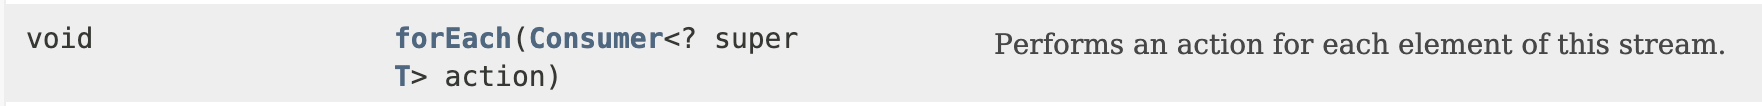
\includegraphics[width=\linewidth]{images/chapter_streams/stream_forEach.png}
  \caption{Methode forEach() in de interface Stream}
  \label{fig:stream_foreach}
\end{figure}

\begin{lstlisting}
public class DemoForEach {

	public static void main(String[] args) {
		Participant john = new Participant("John P.", 15);
		Participant sarah = new Participant("Sarah M.", 200);
		Participant charles = new Participant("Charles B.", 150);
		Participant mary = new Participant("Mary T.", 1);

		List<Participant> participants = Arrays.asList(john, sarah, charles, mary);

		participants.stream()
		    .filter(p -> p.getPoints() >= 200)
		    .forEach(System.out::println);

		System.out.println("* All participants *");

		participants.forEach(System.out::println);
	}
}
\end{lstlisting}

Iedere Collection biedt via de interface Iterable ook een forEach methode aan. Met beide forEach functies kan je hetzelfde resultaat bereiken.

\begin{lstlisting}
participants.forEach(System.out::println);
participants.stream().forEach(System.out::println);
\end{lstlisting}

Toch gaat in dit geval onze voorkeur uit naar de eerste optie. Omdat we hier itereren over alle elementen is de stream overbodig.


\subsection{Intermediate operation .map()}

Als je een functie hebt om objecten van \'e\'en datatype te transformeren naar een ander datatype, dan kan je met de bewerking .map(), deze functie loslaten op alle objecten van een stream. 

\begin{figure}[H]
  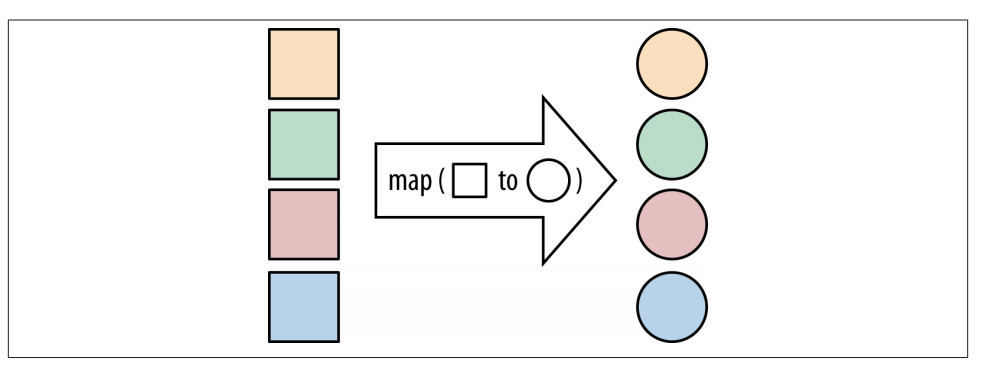
\includegraphics[width=\linewidth]{images/chapter_streams/illustration_map.png}
  \caption{Map operation}
  \label{fig:stream_foreach}
\end{figure}

\begin{figure}[H]
  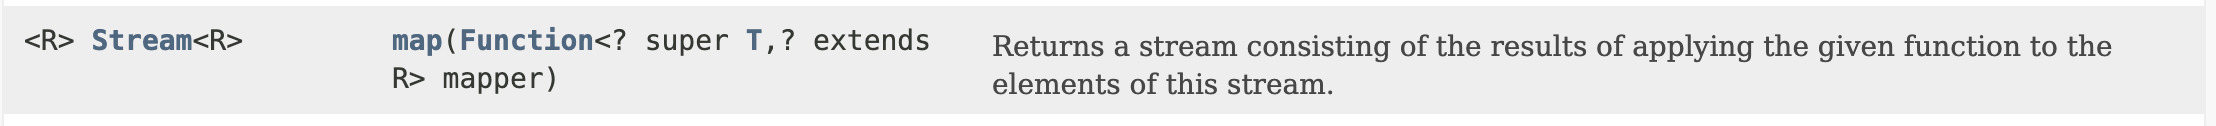
\includegraphics[width=\linewidth]{images/chapter_streams/stream_map.png}
  \caption{Methode map() in de interface Stream}
  \label{fig:stream_foreach}
\end{figure}

Map is een lazy operator. Zonder terminal operator zal de meegegeven functie niet uitgevoerd worden, en zal je dus ook geen resultaat krijgen. De functie die je meegeeft aan map is een implementatie van de generieke functionele interface Function$<$T,R$>$.

Hier volgen een twee voorbeelden. In het eerste voorbeeld wijzigt het datatype van de elementen van de stream niet. In het tweede voorbeeld wordt ieder String-object in de stream vervangen door een Integer-waarde.

\begin{lstlisting}
List<String> animals = Stream.of("zebra", "dog", "dolphine")
				.map(String::toUpperCase)
				.collect(Collectors.toList());

assertEquals(Arrays.asList("ZEBRA", "DOG", "DOLPHINE"), animals);
\end{lstlisting}

\begin{lstlisting}
List<Integer> lengths = Stream.of("zebra", "dog", "dolphine")
				.map(String::length)
				.collect(Collectors.toList());

assertEquals(Arrays.asList(5, 3, 8), lengths);
\end{lstlisting}

\subsection{Intermediate operation .sorted()}

Wanneer je de intermediate operation sorted() toevoegt aan een stream, worden de elementen in de stream gesorteerd. Zonder parameter zal sorted() de natuurlijke sortering gebruiken. Voor objecten van een zelfgeschreven klasse zorg je er dus voor dat de interface Comparable ge\"implementeerd wordt.

Het is ook mogelijk dat je aan de functie sorted() een parameter meegeeft waarmee je een andere volgorde kan afdwingen. In het tweede voorbeeld gebruiken we niet de natuurlijke (alfabetische) volgorde, maar worden de woorden van lang naar kort gesorteerd.


\begin{lstlisting}
List<String> sortedList = Stream.of("zebra", "dog", "dolphine")
				.sorted()
				.collect(Collectors.toList());

assertEquals(Arrays.asList("dog", "dolphine", "zebra"), sortedList);
\end{lstlisting}

\begin{lstlisting}
List<String> sortedList = Stream.of("zebra", "dog", "dolphine")
				.sorted((x, y) -> y.length() - x.length())
				.collect(Collectors.toList());
		
assertEquals(Arrays.asList("dolphine", "zebra", "dog"), sortedList);
\end{lstlisting}

\subsection{Intermediate operation .distinct()}

De operation .distinct() zorgt ervoor dat de elementen in de stream uniek zijn. Elementen die meermaals voorkomen worden verwijderd. Het is de implementatie van de equals() methode (en dus ook hashCode()) van een klasse die beslist of de elementen uniek zijn of niet.

\begin{lstlisting}
List<String> withoutDoubles = Stream.of("zebra", "dog", "zebra", "dolphine")
    .distinct()
    .collect(Collectors.toList());
    
assertEquals(3, withoutDoubles.size());
\end{lstlisting}

\subsection{Intermediate operation .limit()}

De operation .limit() heeft 1 parameter die het maximaal toegelaten elementen in de stream geeft.
De stream wordt dus als het ware afgekapt.

\begin{lstlisting}
List<String> animals = Stream.of("zebra", "dog", "elephant", "camel", "cat", "fish","dolphine")
    .limit(4)
    .collect(Collectors.toList());
assertEquals(4, animals.size());
\end{lstlisting}

Met de methode iterate kunnen we een oneindige stream maken. Dankzij de limit(5) worden slechts de eerste 5 nummers gegenereerd.

\begin{lstlisting}
List<Integer> numbers = Stream.iterate(1, n -> n + n)
    .limit(5)
    .collect(Collectors.toList());

assertEquals(Arrays.asList(1,2,4,8,16), numbers);
\end{lstlisting}


\subsection{Intermediate operation peek()}

De intermediate operation peek kan gebruikt worden om je pipeline te debuggen. Als je wilt controleren welke elementen er op een gegeven moment in de pipeline zitten, dan voeg je peek toe. Zolang je geen terminal operation hebt toegevoegd zal ook peek geen resultaat laten zien.

\begin{lstlisting}
Stream.of("one", "two", "three", "four")
  .filter(e -> e.length() > 3)
  .peek(e -> System.out.println("Filtered value: " + e))
  .map(String::toUpperCase)
  .peek(e -> System.out.println("Mapped value: " + e))
  .collect(Collectors.toList());
\end{lstlisting}

Je kan de operation peek() verder ook handig gebruiken om de elementen van je stream aan te passen.

\begin{lstlisting}
Stream<User> userStream = Stream.of(new User("Alice"), new User("Bob"), new User("Chuck"));
userStream.peek(u -> u.setName(u.getName().toLowerCase()))
  .forEach(System.out::println);
  \end{lstlisting}


\subsection{Terminal operation .count()}

\begin{lstlisting}
long over100Points = participants.stream().filter(p -> p.getPoints() > 100).count();

assertEquals(2, over100Points);
\end{lstlisting}
		
De terminal operation count gebruik je om het aantal elementen in de stream te tellen.
Indien je geen gebruik maakt van intermediate operations gebruik je de methode size() van je collection om het aantal elementen te achterhalen.

\begin{lstlisting}
System.out.println("Number of participants: " + participants.size());
\end{lstlisting}
		
\section{Intstream, LongStream en DoubleStream}
	
Er zijn ook een aantal afgeleide interfaces van de interface Stream. Deze bieden extra functionaliteit aan. Zo hebben we bijvoorbeeld de interface IntStream, die speciaal ontworpen is voor streams met gehele getallen. Deze stream bevat elementen met datatype \textit{int}. Naast IntStream hebben we ook de interfaces DoubleStream en LongStream. Al deze interfaces bevatten de methoden sum(), min(), max() en average(). 

\subsection{sum()}

Met de operation sum kan je eenvoudig de som berekenen van alle elementen in je stream.

\begin{lstlisting}
long totalPoints = participants.stream().mapToInt(Participant::getPoints).sum();

assertEquals(366, totalPoints);
\end{lstlisting}
		

\subsection{range() en rangeClosed()}
		
De static methoden range() en rangeClosed() zijn beschikbaar in de interfaces java.util.stream.IntStream en java.util.stream.LongStream. Je kan ze gebruiken om een stream te cre\"eren met gehele getallen vanaf een init\"ele waarde tot een stop waarde.
\begin{figure}[H]
  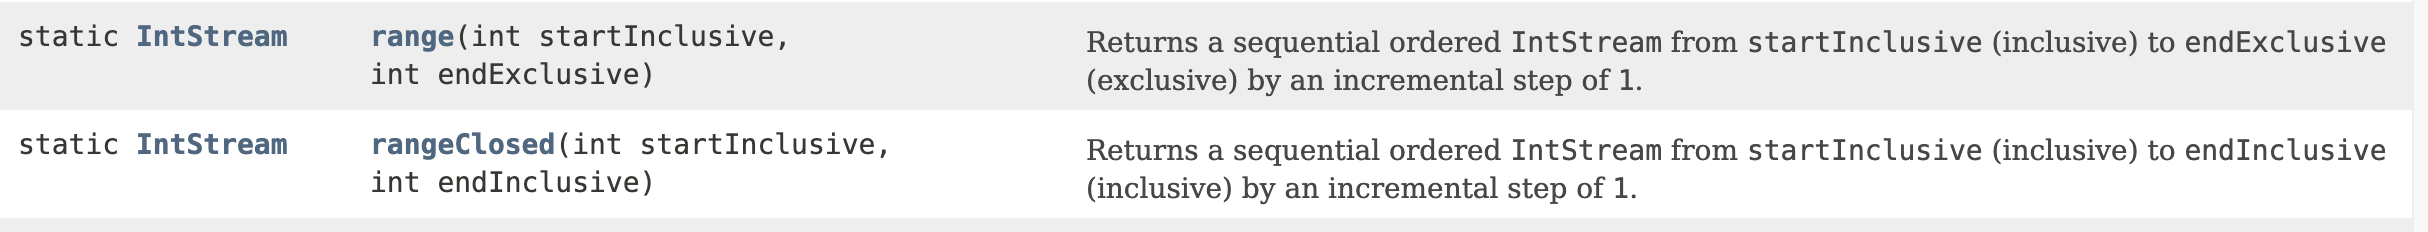
\includegraphics[width=\linewidth]{images/chapter_streams/intstream_range.png}
  \caption{Aanmaken van IntStream met range() of rangeClosed()}
  \label{fig:stream_foreach}
\end{figure}

\begin{lstlisting}
long count = IntStream.rangeClosed(10, 20).count();

assertEquals(11, count);
\end{lstlisting}

\subsection{min(), max() en average()}

\begin{figure}[H]
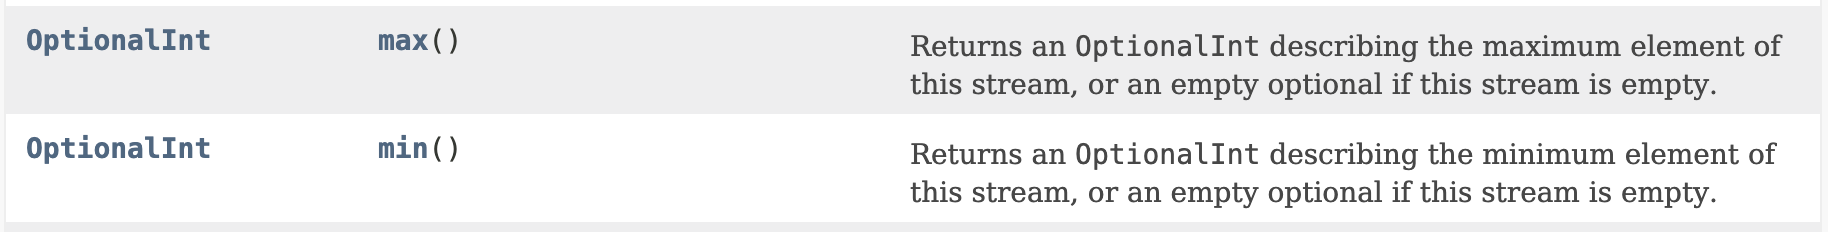
\includegraphics[width=\linewidth]{images/chapter_streams/intstream_max_min.png}
\caption{min() en max() uit de interface IntStream}
\label{fig:instream_min_max}
\end{figure}

\begin{figure}[H]

\includegraphics[width=\linewidth]{images/chapter_streams/intstream_average.png}
\caption{average() uit de interface IntStream}
\label{fig:instream_average}
\end{figure}

Merk op dat de methoden max() en min() een object van de klasse OptionalInt als return-type hebben. De methode average() heeft OptionalDouble als return-type. 

\begin{oefening}
Zoek de klasse OptionalInt en OptionalDouble op in de Java documentatie.
\end{oefening}

In de documentatie vind je terug dat dit een container-object is dat een int- of double-waarde kan bevatten. Indien we namelijk een lege stream hebben, dan bestaat er immers geen minimum, maximum of gemiddelde. In plaats van bijvoorbeeld een exception op te gooien wanneer we max() oproepen voor een lege IntStream, is er gekozen om steeds een OptionalInt als resultaat te geven. Bij een lege IntStream bevat het OptionalIInt-object geen waarde en \textit{isPresent()} geeft false als resultaat. Indien er wel een maximum berekend kan worden geeft \textit{isPresent()} true. De berekende waarde kan je bekomen via de methode \textit{getAsInt()}.

\begin{lstlisting}
Random random = new Random();
List<Integer> randomNumbers = random.ints(15, 0, 100).boxed().collect(Collectors.toList());
int max = randomNumbers.stream().mapToInt(x -> x).max().getAsInt();
int min = randomNumbers.stream().mapToInt(x -> x).min().getAsInt();
double average = randomNumbers.stream().mapToInt(x -> x).average().getAsDouble();
assertTrue(min <= average);
assertTrue(max >= average);

IntSummaryStatistics intSummaryStatistics = random.ints(15, 0, 100).summaryStatistics();
assertTrue(intSummaryStatistics.getMax() >= intSummaryStatistics.getMin());
\end{lstlisting}


\begin{oefening}
Wil je eens aan de slag met de klasse Optional, dan kan je de volgende oefening maken op CodinGame:\\
\url{https://www.codingame.com/playgrounds/20782/java-guild-meeting-52018/optionals---practice}.
\end{oefening}




IMPORTANT THOUGHTS:
- bean scopes
- code quality
source



\section{Components and dependency injection}

All our REST backend applications will consist of 3 layers:
 router-layer (or API-layer), service- or business-layer and persistence-layer.

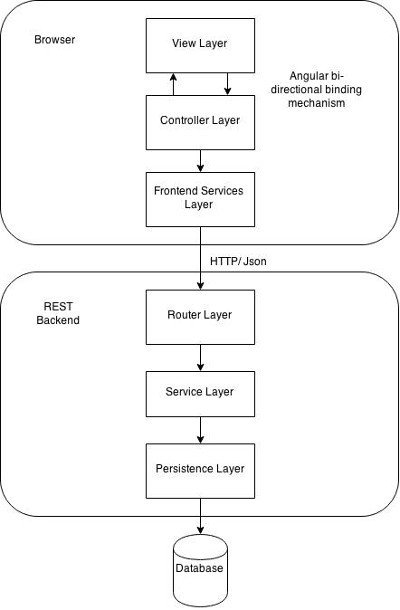
\includegraphics[scale=0.6]{./images/chapter1/spring-architecture.jpeg} 

\begin{itemize}
\item \textbf{Router- or presentation layer:}  Handling and processing HTTP requests,  translating JSON parameters to objects,  authentication of users and protecting data from maleficent users,  ... .
\item \textbf{Service- or business logic layer:} This layer contains the business logic, the core functionality of your application. All calculations, decisions, evaluations, data processing,... are handled by this layer. 
\item \textbf{Data- or persistence layer:} This layer is responsible for interacting with the database.  This layer stores and retrieves the application data in the database.
\end{itemize}

The typical components for each layer are annotated.  These annotated components are managed by Spring. Developers are not responsible for creating the objects of these component classes. The actual objects are created and injected by Spring wherever we need them. In later chapters we will discuss the concept of dependency injection in detail.

The annotations for the Spring components we will use are:
\begin{itemize}
\item @Component: generic annotation for all components managed by Spring
\item @RestController: indicate the components in the API layer
\item @Service: indicate the components in the service layer
\item @Repository: indicate the components in the persistence layer
\end{itemize}

All of these application components (@Component, @Service, @Repository, @Controller, and others) are automatically registered as Spring Beans.

Here is the definition of beans from the Spring framework documentation:

\fcolorbox{black}[HTML]{E9F0E9}{\parbox{\textwidth}{%
\noindent In Spring, the objects that form the backbone of your application and that are managed by the Spring IoC container are called beans. A bean is an object that is instantiated, assembled, and otherwise managed by a Spring IoC container.}}

IoC or Inversion of Control is the process in which an object defines its dependencies without creating them. The IoC container is responsible for constructing the dependencies.

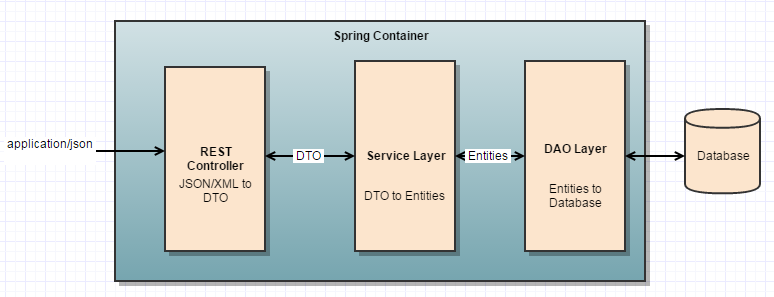
\includegraphics[width=\textwidth]{./images/Spring-REST-Web-Services.png} 

The image shows all the layers that we develop in our REST backend applications. The RestController in the API layer provides REST endpoints. The API layer communicates via DTOs or Data Transfer Objects with the service layer. The service layer implements all business logic. DTOs are mapped to entity-objects and passed along the persistence layer. The persistence layer is responsible for storing the entity-objects in the database.

The Spring container is at the core of the Spring Framework. The container is responsible for creating and managing the objects for classes annotated with @Service, @Repository,... The container will provide these objects (beans) when they are needed by other beans.


\section{DevOps Tools for Java Developers}

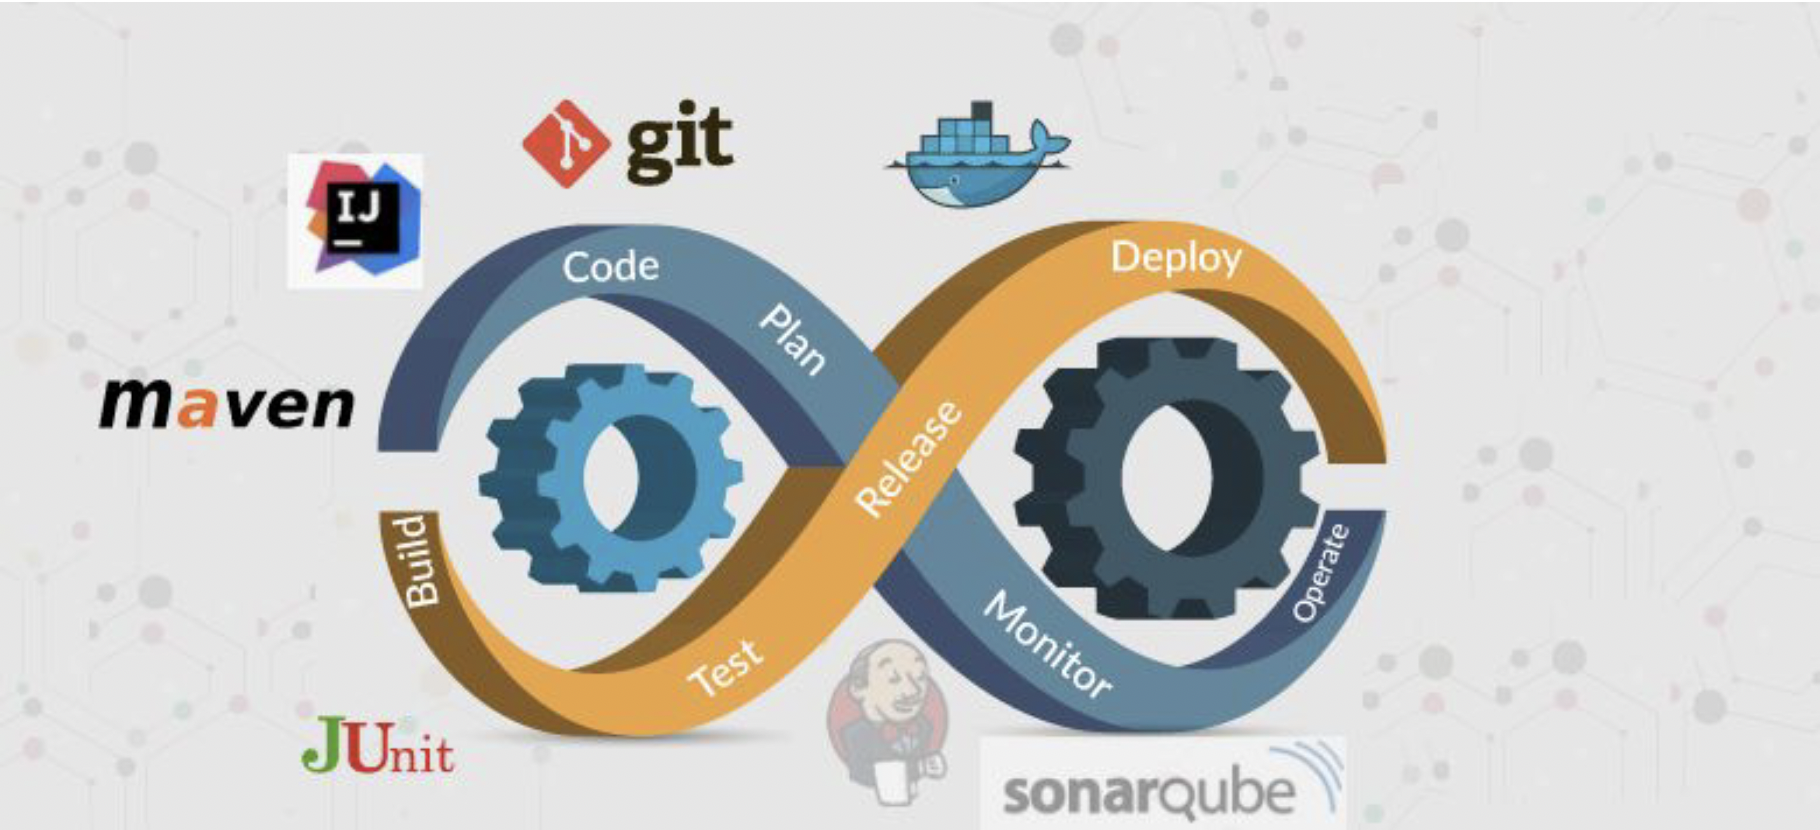
\includegraphics[width=\textwidth]{./images/chapter1/devops.png} 

\printbibliography



\end{document}
